\documentclass[11pt,a4paper]{article}
\usepackage[T1]{fontenc}
\usepackage[utf8]{inputenc}
\usepackage{lmodern,microtype}
\usepackage[margin=26mm]{geometry}
\usepackage{amsmath,amssymb,amsthm,mathtools}
\usepackage{booktabs,array,graphicx,xcolor,tabularx}
\usepackage[colorlinks=true,linkcolor=black,citecolor=black,urlcolor=blue!45!black]{hyperref}
\usepackage{enumitem}
\setlist{itemsep=2pt,topsep=4pt}
\setlength{\emergencystretch}{3em}
\newtheorem{theorem}{Theorem}[section]
\newtheorem{lemma}[theorem]{Lemma}
\newtheorem{corollary}[theorem]{Corollary}
\newtheorem{proposition}[theorem]{Proposition}
\newtheorem{conjecture}[theorem]{Conjecture}
\theoremstyle{definition}
\newtheorem{definition}[theorem]{Definition}
\theoremstyle{remark}
\newtheorem{remark}[theorem]{Remark}
\newcommand{\E}{\mathbb E}
\newcommand{\Pp}{\mathbb P}
\newcommand{\R}{\mathbb R}
\newcommand{\1}{\mathbf 1}
\newcommand{\dd}{\,\mathrm d}
\newcommand{\Kl}{K_{\ell}}
\newcommand{\Kr}{K_{r}}
\newcommand{\kinf}{\kappa_\infty}
\newcommand{\status}[1]{\textsf{[#1]}}
\DeclareMathOperator{\supp}{supp}
\title{Exact exponential moments of interval quasi-stationary laws\\ for L\'evy processes, and the saturation of idealised QSD restart}
\author{Anonymous}
\date{21 October 2026 \quad Version 1.0.0-candidate \quad \href{https://doi.org/10.5281/zenodo.23545672}{doi:10.5281/zenodo.23545672}}
\begin{document}
\maketitle
\begin{abstract}
Restarting a simulation from a quasi-stationary distribution (QSD) is a simple way to look for a rare high level~$L$ of a process that drifts away from it. Its efficiency is governed by an exponential moment of the QSD on the interval $(0,L)$, and Garcia, Bermolen, Jonckheere and Shneer (\emph{Stochastic Systems}, 2026) conjectured that this moment grows like $e^{(\lambda_*-\eta)L}$, where $\lambda_*$ is the Cram\'er root and $\eta$ minimises the cumulant. For L\'evy processes with a Gaussian component and jumps of either sign we prove that every exponential moment $M_L(\theta)$ of the interval QSD has an exact limit after normalisation: bounded below $\eta$ (recovering the half-line formula of Kyprianou and Palmowski), of order $L^2$ at $\eta$, and $\sim C(\theta)e^{(\theta-\eta)L}$ above $\eta$, with constants written through the ladder-height exponents of the Esscher-centred process. The core input is an exact $L^{-2}$ asymptotic for the two boundary layers of the centred QSD. The conjecture therefore holds on the logarithmic scale and up to constants, but its ratio-one reading fails: $C(\lambda_*)<1$ for every spectrally negative process with jumps, $C(\lambda_*)>1$ for every spectrally positive one, and $C(\lambda_*)=0.8501\ldots$ in the source's own example. For idealised QSD restart the success rate is $\sim R_*e^{-\eta L}$ with explicit $R_*$, and the saturation curve $1-\exp(-R_*Be^{-\eta L})$ is accurate uniformly in the budget~$B$ in relative error. Consequently the linear budget regime of the source's restart theorem is $B=O(e^{\eta L})$, not $B=o(e^{\lambda_* L})$. We also extend the moment theorem to spectrally negative processes without a Gaussian component, under a scale-function positivity condition, and, in the source model and conditionally on a regularity property of the QSD density, identify the first-order finite-$L$ corrections: the killing rate sees an effective length $L+\delta_++\delta_-$, where $\delta_\pm$ are the mean stationary overshoots, and both constants carry the relative error $\pi^2(\delta_--\delta_+)/(2L)$.
\end{abstract}

\noindent\textbf{MSC 2020:} Primary 60G51; Secondary 60J25, 60K05, 60F10, 65C05.\\
\textbf{Keywords:} quasi-stationary distribution; L\'evy process; Esscher transform; Wiener--Hopf factorisation; ladder heights; overshoot; restart; rare-event simulation.

%=====================================================================
\section{Introduction}\label{sec:intro}
%=====================================================================

\subsection{The problem in plain terms}\label{sec:plain}
Suppose a simulated process $X$ drifts downwards, and we want to see it reach a high level $L$ at least once within a budget of $B$ units of simulated time. A single run started at $0$ succeeds with probability of order $e^{-\lambda_* L}$, where $\lambda_*>0$ is the Cram\'er root of the cumulant $\psi(s)=\log\E e^{sX_1}$. A \emph{restart} strategy watches each run and, when it falls below a floor (here $0$), discards it and starts afresh from a new point in $(0,L)$. The natural choice of new starting point is a draw from the \emph{quasi-stationary distribution} (QSD) $\nu_L$: the law of $X$ conditioned on having stayed inside $(0,L)$ for a very long time. With this choice the cycles are independent, each lasts an exponential time with rate $\kappa_L$, and each ends at the top with probability $q_L$. The time to first success is therefore exactly exponential with rate $r_L=\kappa_Lq_L$ \cite[Lemma 6.2]{garcia}.

Everything thus hinges on $q_L$. To exit at the top from $y$, the process must climb a distance $L-y$ against its drift, which costs about $e^{-\lambda_*(L-y)}$. Averaging over $y\sim\nu_L$ gives
\[
 q_L\approx e^{-\lambda_* L}\int_0^L e^{\lambda_* y}\,\nu_L(\dd y)=e^{-\lambda_*L}M_L(\lambda_*),
\]
and \cite[Lemma 5.1]{garcia} makes this a two-sided bound. \emph{The efficiency of QSD restart is therefore governed by the exponential moment $M_L(\lambda_*)$ of the QSD.} Garcia et al.\ conjectured that it grows like $e^{(\lambda_*-\eta)L}$, where $\eta$ solves $\psi'(\eta)=0$. This paper determines $M_L(\theta)$ exactly, for every real $\theta$, and draws the consequences for restart.

\emph{Why $\eta$, and not $\lambda_*$, sets the scale.} Conditioning a process to survive for a long time in an interval selects paths with no net drift. The cheapest change of measure that removes the drift is the Esscher tilt by $\eta$, and it weights a position $y$ by $e^{-\eta y}$. So the QSD has density roughly proportional to $e^{-\eta y}$ near the floor, not $e^{-\lambda_* y}$. In $\int e^{\lambda_* y}\nu_L(\dd y)$ the factor $e^{(\lambda_*-\eta)y}$ is largest at the far end, which gives $e^{(\lambda_*-\eta)L}$. The successful-restart rate is then about $e^{-\lambda_*L}e^{(\lambda_*-\eta)L}=e^{-\eta L}$. The point of the paper is to make every step of this sketch exact, including the constants.

\subsection{The source's question, quoted}\label{sec:quote}
We quote the source from its openly accessible version, arXiv:2503.03565v3 \cite{garcia}, and use its numbering; the journal version numbers results consecutively (there, Theorem 3.14 is Theorem 4, Corollary 3.15 is Corollary 2 and Lemma 6.2 is Lemma 5), see Table~\ref{tab:map}. In the source, $x$ is the interval length, $\nu_x$ the QSD on $(0,x)$, $\lambda_0$ the positive root of $\psi'$, and $\tau^{\nu_x}(x)$ the passage time over $x$ of the process restarted from $\nu_x$. After Corollary 3.15 the authors write:
\begin{quote}\small
``For a general L\'evy process, exponential moments of its quasi-stationary measures are not easy to estimate. We conjecture that they grow as $\exp\left[(\lambda^{*}-\lambda_{0})x\right]$, as $x\to+\infty$, where $\lambda_{0}$ is the positive solution of $\psi^{\prime}(\lambda)=0$. Note that this is exactly the case for the linear Brownian motion.''
\end{quote}
The restart theorem whose budget range we revisit is:
\begin{quote}\small
\textbf{Theorem 3.14 of \cite{garcia}.} ``Let $Z$ be a random walk on discrete time or a L\'evy process satisfying (3), (4) and (5) as in Theorem 3.1. For each positive $x\in(0,+\infty)$ let $\nu_{x}$ denote the quasi-stationary probability measure on $(0,x)$ for the process $Z$ absorbed upon exiting $(0,x)$. Let $Z^{\nu_{x}}$ be the restarted version of $Z$ on $(0,x)$ with restart measure $\nu_{x}$ and $\tau^{\nu_{x}}(x)$ the associated passage time over $x$. Let the time budget $B(x)$ grow faster than $x/\psi^{\prime}(\lambda^{*})$ as $x\to+\infty$ but slower than $e^{\lambda^{*}x}$. Then there exist constants $c,C>0$ such that:
\[
c\leq\frac{\Pp(\tau^{\nu_{x}}(x)<B(x))}{\Pp(\tau(x)<B(x))}\cdot\frac{1}{B(x)\int_{0}^{x}e^{\lambda^{*}y}\nu_{x}(dy)}\leq C\qquad(17)
\]
for all $x>0$.''
\end{quote}
Its Brownian specialisation, Corollary 3.15, states that for drift $-\mu$ one has $\int_0^xe^{\lambda^*y}\nu_x(dy)=e^{\mu x}$ and that the ratio in (17), with this moment, ``is bounded away from zero and infinity for $B(x)$ growing faster than $x/\mu$''. The cited lemmas are: Lemma 5.1, which defines $q(x)=\Pp_{\nu_x}(\tau(x)<\tau(0))$ and proves $c\int_0^xe^{\lambda^*y}\nu_x(dy)\le e^{\lambda^*x}q(x)\le\int_0^xe^{\lambda^*y}\nu_x(dy)$; Lemma 6.1, convergence of $\nu_x$ to the half-line Yaglom limit; and Lemma 6.2, the exponential law of $\tau^{\nu_x}(x)$ with parameter $\beta(x)q(x)$.

\begin{table}[t]
\centering\small
\caption{Notation map between the source \cite{garcia} and this paper.}\label{tab:map}
\begin{tabularx}{\textwidth}{@{}Xp{.36\textwidth}p{.27\textwidth}@{}}
\toprule
Object & Source (arXiv v3; journal version) & This paper\\
\midrule
interval length & $x$ & $L$\\
QSD on the interval & $\nu_x$ & $\nu_L$\\
root of $\psi'$ & $\lambda_0$ & $\eta$\\
Cram\'er root & $\lambda^*$ & $\lambda_*$\\
absorption rate of the QSD & $\beta(x)$ & $\kappa_L$\\
upper-exit probability of a QSD cycle & $q(x)$ & $q_L$\\
budget & $B(x)$ & $B$ or $B_L$\\
Brownian drift & $-\mu$ & $-m$\\
cycle-duration variable (source Lemma 5.2) & $\eta$ & not used\\
\midrule
restart theorem & Thm 3.14; Thm 4 & Theorem~\ref{thm:restart}, Corollary~\ref{cor:corrected}\\
Brownian corollary / conjecture & Cor 3.15 and the paragraph after it; Cor 2 & \S\ref{sec:verdict}\\
Yaglom convergence; exponential restart law & Lemmas 6.1, 6.2; Lemma 5 (for 6.2) & Cor~\ref{cor:consequences}(ii), \eqref{eq:restart-exact}\\
\bottomrule
\end{tabularx}
\end{table}

\subsection{The answer, reading by reading}\label{sec:verdict}
The conjecture's phrase ``grow as'' admits several readings. Table~\ref{tab:verdict} gives our verdict on each; $C_*$ denotes the limit of $e^{-(\lambda_*-\eta)L}M_L(\lambda_*)$, which exists and is identified in Theorem~\ref{thm:main}.

\begin{table}[h]
\centering\small
\caption{Verdict on each reading of the conjecture (processes with a Gaussian component; spectrally negative processes also without, Theorem~\ref{thm:sn}).}\label{tab:verdict}
\begin{tabularx}{\textwidth}{@{}p{.33\textwidth}Xl@{}}
\toprule
Reading & Verdict & Where\\
\midrule
logarithmic: $L^{-1}\log M_L(\lambda_*)\to\lambda_*-\eta$ & true & Thm~\ref{thm:main}\\
two-sided: $M_L(\lambda_*)\asymp e^{(\lambda_*-\eta)L}$ & true & Thm~\ref{thm:main}\\
ratio limit with some constant & true, with explicit $C_*\in(0,\infty)$ & Thm~\ref{thm:main}\\
ratio one: $M_L(\lambda_*)\sim e^{(\lambda_*-\eta)L}$ ``exactly'' as for Brownian motion & \textbf{false in general}: $C_*=1$ for Brownian motion, $C_*<1$ for every spectrally negative and $C_*>1$ for every spectrally positive process with jumps; $C_*=0.8501\ldots$ in the source's example & Prop~\ref{prop:ratioone}\\
\bottomrule
\end{tabularx}
\end{table}

\subsection{Heuristic picture}\label{sec:heuristic}
After the Esscher tilt by $\eta$ the process $Y$ has mean zero, and its QSD $\widetilde\nu_L$ on $(0,L)$ is related to $\nu_L$ by $\nu_L(\dd y)\propto e^{-\eta y}\widetilde\nu_L(\dd y)$. A centred process confined to a long interval looks diffusive, so $\widetilde\nu_L$ has a \emph{sine-shaped bulk}, $\widetilde\nu_L(L\dd u)\approx\frac\pi2\sin(\pi u)\dd u$, carrying mass of order one. Near each end the sine vanishes linearly, and at distance $O(1)$ from the end the jumps matter: the density there forms a \emph{boundary layer} of height $O(L^{-2})$, whose shape is the renewal function of the ladder heights of $Y$ (ascending at the left end, descending at the right end):
\[
 \widetilde\nu_L(\dd y)\approx\frac{\pi^2}{2L^2}\,m_+V_+(y)\dd y\ \ (y=O(1)),\qquad
 \widetilde\nu_L(L-\dd y)\approx\frac{\pi^2}{2L^2}\,m_-V_-(y)\dd y\ \ (y=O(1)).
\]
Figure~\ref{fig:layers} shows both layers for the source's model. Every exponential moment is a ratio of two Laplace transforms of $\widetilde\nu_L$,
\[
 M_L(\theta)=\frac{\int e^{(\theta-\eta)y}\widetilde\nu_L(\dd y)}{\int e^{-\eta y}\widetilde\nu_L(\dd y)}.
\]
The denominator only sees the left layer, so it is $L^{-2}$ times a constant. For $\theta>\eta$ the numerator only sees the right layer, so it is $e^{(\theta-\eta)L}L^{-2}$ times a constant. The factors $L^{-2}$ cancel and leave $C(\theta)e^{(\theta-\eta)L}$. For $\theta<\eta$ both see the left layer and the ratio is $O(1)$; at $\theta=\eta$ the numerator is $1$ and the ratio is of order $L^2$. The constants are Laplace transforms of the two renewal profiles, and Wiener--Hopf factorisation turns them into the closed forms of Theorem~\ref{thm:main}. The jump-free case makes the picture concrete: for Brownian motion with drift the layers are exactly linear, $V_\pm(y)\propto y$, and $C_*=1$.

\begin{figure}[t]
\centering
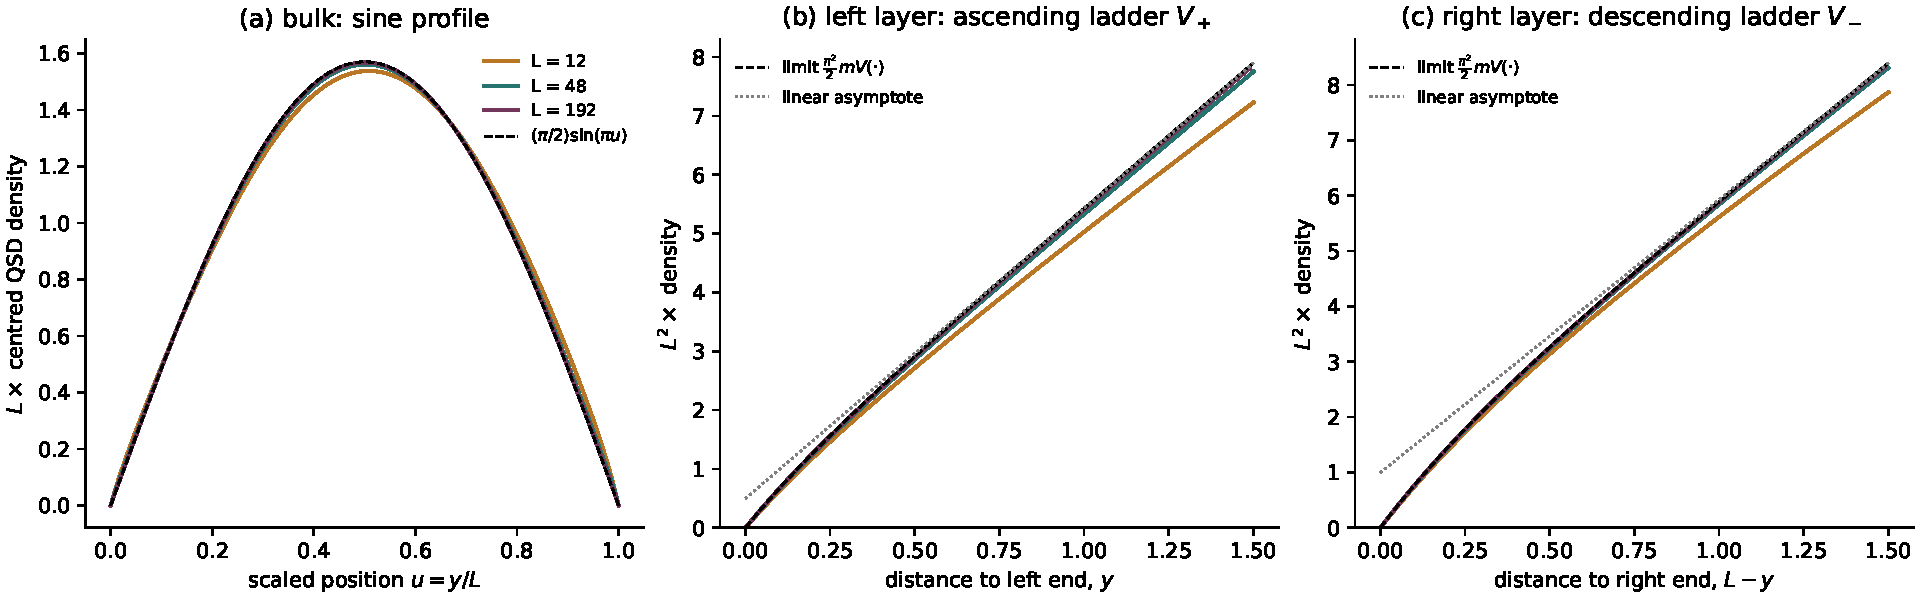
\includegraphics[width=\textwidth]{checks/boundary_layers.pdf}
\caption{Centred QSD of the source's two-sided exponential-jump model (exact finite-interval solution). (a) Bulk: $L$ times the density against $u=y/L$ approaches $\frac\pi2\sin(\pi u)$. (b), (c) Boundary layers: $L^2$ times the density near each end approaches $\frac{\pi^2}{2}m_\pm V_\pm$ (dashed), which bends away from its linear asymptote $\frac{\pi^2}{2}(y+\delta_\pm)$ (dotted). The offsets $\delta_\pm$ are the mean stationary overshoots, which reappear as an effective-length shift in \S\ref{sec:finiteL}. Numerical illustration only.}
\label{fig:layers}
\end{figure}

\subsection{Contributions}\label{sec:contrib}
Table~\ref{tab:contrib} lists what is proved and how each statement is supported. We use four labels throughout: \status{proof} (complete written proof); \status{certified} (exact or outward-rounded interval arithmetic); \status{numerical} (high-precision computation, not a proof); \status{exploratory} (conjecture or heuristic supported by computation).

\begin{table}[h]
\centering\small
\caption{Results, their role, and their support.}\label{tab:contrib}
\begin{tabularx}{\textwidth}{@{}Xp{.33\textwidth}l@{}}
\toprule
Statement & Role & Label\\
\midrule
\multicolumn{3}{@{}l}{\emph{Core results}}\\
Exact $L^{-2}$ endpoint masses of the centred QSD (Thm~\ref{thm:endpoint}) & the main technical result & \status{proof}\\
Critical and supercritical moments, constant $C(\theta)$, $C_*$ (Thm~\ref{thm:main}) & answers the conjecture with constants & \status{proof}\\
Restart rate $r_L\sim R_*e^{-\eta L}$ (Thm~\ref{thm:restart}) & constant for the source's restart law & \status{proof}\\
\multicolumn{3}{@{}l}{\emph{Consequences}}\\
Ratio-one reading false; sign of $C_*-1$ for one-sided jumps (Prop~\ref{prop:ratioone}) & settles the strong reading & \status{proof}, \status{certified}\\
Uniform relative-error saturation curve (Thm~\ref{thm:restart}(iii)) & usable at all budgets & \status{proof}\\
Corrected budget range $B=O(e^{\eta L})$ of source Thm 3.14 (Cor~\ref{cor:corrected}) & correction of a published statement & \status{proof}\\
Spectrally negative processes without Gaussian part (Thm~\ref{thm:sn}) & one step beyond $\sigma>0$, under scale-function condition (Q); pure-jump example conditional on (Q) & \status{proof}, \status{numerical}\\
First-order $1/L$ correction in the source model (Thms~\ref{thm:e1-alpha}, \ref{thm:e1-CR}) & effective length, finite-$L$ accuracy & \status{proof}\textsuperscript{a}\\
\multicolumn{3}{@{}l}{\emph{Recovered or standard, included for completeness}}\\
Subcritical moments $\theta<\eta$ & half-line formula of \cite{kypalm} via \cite[Lemma 6.1]{garcia} & \status{proof}\\
Sine law and $\kappa_L=\kinf+\pi^2v/(2L^2)+o(L^{-2})$ & standard diffusive scaling; closely related to \cite{lotovkh} & \status{proof}\\
Large deviations of $X/L$, transition window $\theta=\eta+z/L$ & immediate corollaries & \status{proof}\\
General effective-length conjecture (Conj~\ref{conj:general}) & open & \status{exploratory}\\
\bottomrule
\end{tabularx}\\[2pt]
\raggedright\footnotesize\textsuperscript{a}\,Conditional on the regularity property (F1) of \S\ref{sec:finiteL}, which is not proved; second-order constants are \status{numerical}.
\end{table}

What the exact constant adds beyond the two-sided reading deserves a sentence. Combining the source's Lemma 5.1 with the stopped identity \eqref{eq:rate-transform} below reduces $M_L(\lambda_*)\asymp e^{(\lambda_*-\eta)L}$ to two-sided bounds $\alpha_L\asymp L^{-2}$ and $\int e^{-\eta y}\widetilde\nu_L(\dd y)\asymp L^{-2}$, which ground-state estimates could plausibly supply. The ratio limit does more: it gives the restart constant $R_*$ and hence the budget needed for a prescribed success probability (\S\ref{sec:practice}); it locates the exact budget range of the source's theorem (Cor.~\ref{cor:corrected}); it shows that the strong reading of the conjecture fails and that $C_*-1$ measures the asymmetry of the jumps (Prop.~\ref{prop:ratioone}); and it is the starting point for the finite-$L$ correction (\S\ref{sec:finiteL}).

\subsection{Related work and positioning}\label{sec:related}
\emph{Quasi-stationarity of L\'evy processes.} For a fixed interval, existence, uniqueness and exponential convergence to the QSD are due to Kolb and Savov \cite{kolbsavov}; for spectrally one-sided processes Bertoin \cite{bertoin97} and Lambert \cite{lambert} describe the principal eigenvalue and eigenfunctions through scale functions. On the half-line, Kyprianou and Palmowski \cite{kypalm} identify the Yaglom limit after an Esscher tilt, with a density built from a ladder renewal function. Our subcritical regime $\theta<\eta$ recovers their formula, through the interval-to-half-line convergence proved in \cite[Lemma 6.1]{garcia} with the first-passage asymptotics of Denisov and Shneer \cite{denisovshneer}; the Brownian case goes back to Mart\'inez and San Mart\'in \cite{martinezsm}. General background is in \cite{cms,melvill}, and \cite{champvill} gives a general framework for exponential convergence to QSDs. What the present paper adds is the behaviour at and above $\eta$: the exact $L^{-2}$ normalisation of both boundary layers (Theorem~\ref{thm:endpoint}), which the half-line limit cannot see, and the constants $C(\theta)$ and $R_*$ it determines.

\emph{Two-boundary problems and large intervals.} Exit problems for an interval have a long history. Exact transforms of the two-sided exit time and overshoot are available for spectrally one-sided processes \cite{bertoin97,lambert} and for particular classes of L\'evy processes with exponential-type jumps \cite{kadver}. Exact one-sided first-passage identities for L\'evy processes with two-sided phase-type jumps, a class containing the source's model, are in \cite{aap}. Asymptotic expansions for the exit from a widening interval, under Cram\'er-type conditions, were developed by Lotov and coauthors for random walks and processes with independent increments \cite{lotov79,lotovkh,lotov16,khodzhibaev14}. They cover the asymptotics of the exit-side probabilities and of Laplace transforms of the exit time as the interval grows, including the diffusive regime after an exponential change of measure. We have read only the zbMATH reviews of \cite{lotovkh,khodzhibaev14} and could not access \cite{lotov79,lotov16} in full. We did not find the expansion $\kappa_L=\kinf+\pi^2v/(2L^2)+o(L^{-2})$ stated there, but we regard it, and the exit-side limit $Q_L\to1/2$ of Lemma~\ref{lem:exit}, as closely related to and plausibly implied by that work; we claim neither. Nothing we read there concerns endpoint masses or exponential moments of the QSD. For diffusions with killing, quasi-limiting behaviour is classical \cite{mandl,kolbst}.

On the analytic side, the principal eigenvalue of nonlocal operators on large domains scales diffusively (Garc\'ia-Meli\'an and Rossi \cite{garciarossi} for symmetric kernels; Du, Fang and Ni \cite{du} for asymmetric kernels), interval exit times are comparable with products of ladder renewal functions (Grzywny \cite{grzywny}), and convolution equations on large intervals have interior trigonometric profiles with endpoint corrections in the Wiener--Hopf tradition (Ponomarev \cite{ponomarev} and references there). We therefore do not regard the sine bulk, the $L^{-2}$ eigenvalue correction or the renewal shape of the boundary layers as new in themselves; Corollary~\ref{cor:consequences}(i) is included because the proof needs it. The fluctuation-theoretic inputs (Wiener--Hopf factorisation, Vigon's \'equation amicale, stationary overshoots) are classical \cite{bertoinbook,doney,kyprianoubook,vigon,bvhs,doring}.

\emph{Restart, resetting and splitting.} ``Restart'' has several meanings. In rare-event simulation, RESTART names a multilevel splitting method \cite{villen}, which is different from the exit-triggered QSD restart studied here; splitting, adaptive multilevel splitting and go-with-the-winners schemes \cite{ghsz,cerougu,cdgr,aldousvaz} are the natural benchmarks (\S\ref{sec:practice}). Restart strategies for randomised algorithms \cite{lsz} and stochastic resetting in statistical physics \cite{evansmaj,palreuveni} usually reset to a fixed state at chosen times (for L\'evy flights escaping an interval under resetting, see \cite{zbik}); exploration methods in reinforcement learning restart from archived promising states \cite{goexplore}. Fleming--Viot particle systems \cite{bhm,ferrarimaric,villemonais14,afg,cdgrfv} are the standard way to approximate a QSD, and \cite{garcia} discusses them as the practical motivation.


\subsection{Roadmap}
Section~\ref{sec:results} fixes notation (Table~\ref{tab:notation}) and states all results. Section~\ref{sec:diffusive} proves the sine law; Section~\ref{sec:boundary} proves the endpoint-mass theorem, which is the heart of the paper; Section~\ref{sec:moment-proof} deduces the moment theorem and its corollaries; Section~\ref{sec:restart-proof} treats restart and the corrected budget range; Section~\ref{sec:ratioone-proof} the ratio-one reading; Section~\ref{sec:sn} spectrally negative processes without a Gaussian component; Section~\ref{sec:finiteL} the finite-$L$ correction; Section~\ref{sec:examples} exact examples and numerical checks; Section~\ref{sec:practice} consequences for simulation practice; Section~\ref{sec:open} open problems.

%=====================================================================
\section{Setting, notation and results}\label{sec:results}
%=====================================================================

\subsection{Hypotheses and standing facts}
Let $X$ be a real L\'evy process with Gaussian coefficient $\sigma>0$ and L\'evy measure $\Pi$, and let $\psi(s)=\log\E e^{sX_1}$. We assume
\begin{equation}\label{eq:H}\tag{H}
 \psi(s)<\infty\ \text{ for } 0\le s<s_{\max},\qquad 0<\lambda_*<s_{\max},\qquad \psi(\lambda_*)=0,
\end{equation}
for some $s_{\max}\in(0,\infty]$. These are the source's Gaussian and Cram\'er assumptions for L\'evy processes. As $\psi$ is strictly convex with $\psi(0)=\psi(\lambda_*)=0$, it is negative on $(0,\lambda_*)$ and has a unique minimiser $\eta\in(0,\lambda_*)$. Put
\begin{equation}\label{eq:parameters}
 \kinf=-\psi(\eta)>0,\qquad v=\psi''(\eta)>0,\qquad \chi(s)=\psi(\eta+s)-\psi(\eta).
\end{equation}
The \emph{centred Esscher law} $\widetilde\Pp$ is defined, for $X_0=y$, by
\begin{equation}\label{eq:esscher}
 \frac{\dd\widetilde\Pp_y}{\dd\Pp_y}\bigg|_{\mathcal F_t}=\exp\{\eta(X_t-y)-t\psi(\eta)\}.
\end{equation}
Under $\widetilde\Pp$ we write $Y$ for the process. We use the following standard facts.
\begin{enumerate}[label=(S\arabic*),leftmargin=*]
\item $Y$ is a L\'evy process with Gaussian coefficient $\sigma$, L\'evy measure $\widetilde\Pi(\dd x)=e^{\eta x}\Pi(\dd x)$ and cumulant $\chi$, finite on $(-\eta,s_{\max}-\eta)$. Hence $\E Y_1=\chi'(0)=0$ and $\operatorname{Var}Y_1=v$. No negative exponential moment of $X$ is assumed: on $(-\infty,-1)$, $e^{-\eta x}\widetilde\Pi(\dd x)=\Pi(\dd x)$ has finite mass.
\item $Y$ oscillates, so its ascending and descending ladder-height processes $H_+$, $H_-$ are unkilled subordinators. We normalise their local times so that the Wiener--Hopf factorisation reads (\cite[Ch.~6]{kyprianoubook}; \cite{doney})
\begin{equation}\label{eq:wh}
 \chi(s)=-\phi_+(-s)\phi_-(s),\qquad \E e^{-qH_\pm(t)}=e^{-t\phi_\pm(q)},
\end{equation}
first on the imaginary axis and then on the real strip where $\chi$ is finite. One normalisation constant remains free; every constant in this paper is invariant under it.
\item The drifts $d_\pm$ of $H_\pm$ satisfy $d_+d_-=\sigma^2/2$ (\cite{doney}; \cite[Thm 5.3]{doring} in Markov-additive form), so $d_\pm>0$. The L\'evy measures $\Pi_\pm$ of $H_\pm$ are given by Vigon's \'equation amicale \cite{vigon,doney}:
\begin{equation}\label{eq:vigon}
 \Pi_+(\dd z)=\int_{[0,\infty)}U_-(\dd y)\,\widetilde\Pi(y+\dd z),\qquad z>0,
\end{equation}
and symmetrically for $\Pi_-$, where $U_\pm(\dd y)=\int_0^\infty\Pp(H_\pm(t)\in\dd y)\dd t$ are the renewal measures.
\item The means $m_\pm=\E H_\pm(1)=\phi'_\pm(0+)$ are finite and positive, and $m_+m_-=v/2$ (Lemma~\ref{lem:ladder}).
\item Ladder exponential moments are inherited from the parent: for $0<s<s_{\max}-\eta$ and $0<s\le\eta$ respectively,
\begin{equation}\label{eq:ladder-exp}
\begin{aligned}
 \int_{(1,\infty)}e^{sz}\Pi_+(\dd z)&\le\frac{1}{d_-s}\int_{(1,\infty)}e^{sx}\widetilde\Pi(\dd x)<\infty,\\
 \int_{(1,\infty)}e^{sz}\Pi_-(\dd z)&\le\frac{1}{d_+s}\int_{(-\infty,-1)}e^{-sx}\widetilde\Pi(\dd x)<\infty.
\end{aligned}
\end{equation}
\end{enumerate}
Let $\tau_L=\inf\{t\ge0:X_t\notin(0,L)\}$. The process killed at $\tau_L$ has a unique QSD for each $L$ (\cite[Thm 2.1, Remark 2.2]{kolbsavov}; see also the remark after Table~\ref{tab:notation}): $\nu_L$ under $\Pp$ with killing rate $\kappa_L$, and $\widetilde\nu_L$ under $\widetilde\Pp$ with killing rate $\alpha_L$, so that
\[
 \Pp_{\nu_L}(\tau_L>t)=e^{-\kappa_Lt},\qquad \Pp_{\nu_L}(X_t\in\Gamma\mid\tau_L>t)=\nu_L(\Gamma),
\]
and likewise for $\widetilde\nu_L$, $\alpha_L$.

\begin{table}[t]
\centering\small
\caption{Notation. Each symbol has one meaning throughout.}\label{tab:notation}
\begin{tabularx}{\textwidth}{@{}lX@{}}
\toprule
$\psi,\ \lambda_*,\ \eta$ & cumulant of $X$; Cram\'er root $\psi(\lambda_*)=0$; minimiser $\psi'(\eta)=0$\\
$\kinf,\ v,\ \chi$ & $-\psi(\eta)$; $\psi''(\eta)$; centred cumulant $\chi(s)=\psi(\eta+s)-\psi(\eta)$\\
$\widetilde\Pp,\ Y,\ \widetilde\Pi$ & Esscher-centred law, the process under it, its L\'evy measure\\
$\tau_L$ & exit time from $(0,L)$\\
$\nu_L,\ \kappa_L$ & QSD and killing rate of $X$ on $(0,L)$\\
$\widetilde\nu_L,\ \alpha_L$ & QSD and killing rate of $Y$ on $(0,L)$; $\kappa_L=\kinf+\alpha_L$\\
$A_L(s)$ & $\int e^{sy}\widetilde\nu_L(\dd y)$, finite for all real $s$\\
$M_L(\theta)$ & $\int e^{\theta y}\nu_L(\dd y)=A_L(\theta-\eta)/A_L(-\eta)$\\
$H_\pm,\ \phi_\pm,\ d_\pm,\ \Pi_\pm$ & ascending/descending ladder heights of $Y$, their exponents, drifts, L\'evy measures\\
$U_\pm,\ V_\pm,\ m_\pm$ & renewal measures, renewal functions $V_\pm(y)=U_\pm([0,y])$, means $\phi_\pm'(0)$\\
$O_a^\pm$ & overshoot of $Y$ (from $0$) above $a$, resp.\ magnitude of undershoot below $-a$\\
$\rho_\pm,\ G_\pm,\ \delta_\pm$ & stationary overshoot laws, their transforms $G_\pm(s)=\int e^{sz}\rho_\pm(\dd z)$, means $\delta_\pm=\int z\rho_\pm(\dd z)$\\
$\Kl(b),\ \Kr(b)$ & endpoint constants $\pi^2m_+/(2b\phi_+(b))$, $\pi^2m_-/(2b\phi_-(b))$, $b>0$\\
$C(\theta),\ C_*$ & $\Kr(\theta-\eta)/\Kl(\eta)$ for $\theta>\eta$; $C_*=C(\lambda_*)$\\
$q_L,\ r_L,\ R_*$ & upper-exit probability of a QSD cycle; restart rate $\kappa_Lq_L$; its constant\\
$p^{\mathrm R}_L(B),\ p^0_L(B)$ & success probability within budget $B$: QSD restart; single run from $0$\\
$\Gamma$ & a Borel set\\
$a_\pm,\ \beta_\pm,\ k_\pm$ & (source example only, \S\ref{sec:source}) roots, tilted jump rates, ladder normalisations\\
\bottomrule
\end{tabularx}
\end{table}

\begin{remark}[Existence, uniqueness and full support]\label{rem:support}
For fixed $L$ the killed process has a unique QSD by \cite[Thm 2.1 and Remark 2.2]{kolbsavov}, whose hypothesis (absolute continuity of the law of $X_t$ for $t>0$) holds because $\sigma>0$. The QSD charges every open interval $J\subset(0,L)$. Indeed $\widetilde\nu_L(J)=e^{\alpha_Lt}\int\widetilde\nu_L(\dd x)\widetilde\Pp_x(Y_t\in J,\tau_L>t)$, and $\widetilde\Pp_x(Y_t\in J,\tau_L>t)>0$ for each $x\in(0,L)$. To see the latter, fix a continuous path $f$ from $x$ into $J$ staying at distance at least $2\varepsilon$ from $\{0,L\}\cup J^c$ at the end. Write $Y=\sigma W+Z$ with $W$ a Brownian motion independent of the jump part $Z$. With positive probability $Z$ has no jump of size larger than $\varepsilon'$ on $[0,t]$; on that event $Z_s=b's+N_s$ for a constant $b'$ and a square-integrable martingale $N$ with $\E\sup_{s\le t}N_s^2\le4t\int_{|z|\le\varepsilon'}z^2\widetilde\Pi(\dd z)$, which is below $\varepsilon^2/8$ for small $\varepsilon'$; by Doob's inequality $\sup_{s\le t}|N_s|<\varepsilon$ with conditional probability at least $1/2$. Independently, $\sup_{s\le t}|x+\sigma W_s+b's-f(s)|<\varepsilon$ with positive probability by the support theorem for Brownian motion. On the intersection, $Y$ stays in $(0,L)$ and ends in $J$.
\end{remark}

\subsection{Main results}
\begin{theorem}[Exact moment asymptotics]\label{thm:main}
Under \eqref{eq:H},
\begin{equation}\label{eq:moment-main}
\begin{aligned}
 \lim_{L\to\infty}M_L(\theta)&=\frac{\Kl(\eta-\theta)}{\Kl(\eta)}, &&\theta<\eta,\\
 \lim_{L\to\infty}L^{-2}M_L(\eta)&=\frac1{\Kl(\eta)},\\
 \lim_{L\to\infty}e^{-(\theta-\eta)L}M_L(\theta)&=C(\theta), &&\theta>\eta,
\end{aligned}
\end{equation}
with $C(\theta)=\Kr(\theta-\eta)/\Kl(\eta)\in(0,\infty)$. In particular $L^{-1}\log M_L(\theta)\to(\theta-\eta)_+$ for every real $\theta$, and the conjectured moment satisfies
\begin{equation}\label{eq:conjecture-solution}
 M_L(\lambda_*)\sim C_*e^{(\lambda_*-\eta)L},\qquad
 C_*=\frac{\Kr(\lambda_*-\eta)}{\Kl(\eta)}=\frac{G_+(\lambda_*-\eta)}{G_-(\eta)}.
\end{equation}
\end{theorem}
Here $\sim$ means that the ratio tends to one. The theorem holds for every fixed real $\theta$, including $\theta\ge s_{\max}$, where $M_L(\theta)$ is finite only because the interval is bounded. It is a pointwise statement in $\theta$; the only uniform statement is the window in Corollary~\ref{cor:consequences}(iii).

The engine of Theorem~\ref{thm:main} is the following description of the two boundary layers of the centred QSD.
\begin{theorem}[Endpoint masses of the centred QSD]\label{thm:endpoint}
For every $b>0$,
\begin{equation}\label{eq:boundary-laplace}
 L^2A_L(-b)\longrightarrow\Kl(b),\qquad L^2e^{-bL}A_L(b)\longrightarrow\Kr(b).
\end{equation}
Equivalently, extending each measure by zero to $[0,\infty)$,
\begin{equation}\label{eq:weighted-boundary}
 L^2e^{-by}\widetilde\nu_L(\dd y)\Rightarrow\frac{\pi^2m_+}{2}e^{-by}V_+(y)\dd y,\qquad
 L^2e^{-by}\widetilde\nu_L(L-\dd y)\Rightarrow\frac{\pi^2m_-}{2}e^{-by}V_-(y)\dd y.
\end{equation}
\end{theorem}

\begin{remark}[Which ladder sits at which end]\label{rem:orientation}
The left layer is shaped by the \emph{ascending} ladder of $Y$, and the right one by the descending ladder. This is the most error-prone point of the construction: with the orientations swapped, the source model would give $C_*\approx1.2926$ instead of $0.8501$, a value excluded by the exact finite-$L$ solution in \S\ref{sec:source}. Heuristically, the QSD density $p$ is a \emph{left} eigenfunction: it solves the forward equation, whose generator is that of the dual process $\widehat Y=-Y$. Near the left end, $\alpha_L\approx0$ and $p$ is approximately harmonic for $\widehat Y$ killed on entering $(-\infty,0]$. Such harmonic functions are renewal functions of the descending ladder height of $\widehat Y$, which is the ascending ladder height of $Y$. The proof below does not use this heuristic: the orientation is fixed by the exact identities of Lemma~\ref{lem:dynkin} and the Wiener--Hopf cancellation \eqref{eq:cancellation}.
\end{remark}

\begin{corollary}[Recovered and immediate consequences]\label{cor:consequences}
Under \eqref{eq:H}:
\begin{enumerate}[label=(\roman*)]
\item $L^2\alpha_L\to\pi^2v/2$, so $\kappa_L=\kinf+\pi^2v/(2L^2)+o(L^{-2})$; and $\widetilde\nu_L(L\dd u)\Rightarrow\frac\pi2\sin(\pi u)\1_{(0,1)}(u)\dd u$.
\item $\nu_L\Rightarrow\eta\phi_+(\eta)e^{-\eta y}V_+(y)\dd y$, the half-line Yaglom law of \cite[Theorem 1]{kypalm}; and $\Kl(\eta-\theta)/\Kl(\eta)=\eta\phi_+(\eta)/((\eta-\theta)\phi_+(\eta-\theta))$ for $\theta<\eta$.
\item Uniformly for $z$ in compact subsets of $\R$, $L^{-2}M_L(\eta+z/L)\to\pi^2(1+e^z)/(2\Kl(\eta)(z^2+\pi^2))$.
\item The laws of $X/L$ under $\nu_L$ satisfy a large-deviation principle on $[0,1]$ with speed $L$ and rate $I(u)=\eta u$.
\end{enumerate}
\end{corollary}

\subsection{Idealised QSD restart}
Start from $\nu_L$; stop at the first exit above $L$; after each exit below $0$ draw a fresh independent point from $\nu_L$ and continue. Let $p^{\mathrm R}_L(B)$ be the probability of an upper exit within total simulated time $B$, and $q_L=\Pp_{\nu_L}(X_{\tau_L}\ge L)$. Restart draws are free and exits are monitored continuously.
\begin{theorem}[Restart rate and saturation]\label{thm:restart}
Under \eqref{eq:H}:
\begin{enumerate}[label=(\roman*)]
\item \textup{(exact law, \cite[Lemma 6.2]{garcia})} $p^{\mathrm R}_L(B)=1-e^{-r_LB}$ for all $B\ge0$, with $r_L=\kappa_Lq_L$;
\item $r_L\sim R_*e^{-\eta L}$ with
\begin{equation}\label{eq:restart-rate}
 R_*=\frac{m_-}{m_+}\phi_+(\eta)^2=\kinf\frac{G_+(-\eta)}{G_-(\eta)}\in(0,\infty);
\end{equation}
\item \textup{(uniform relative error)} with $a_L=r_Le^{\eta L}/R_*\to1$, for every $L$,
\begin{equation}\label{eq:uniform-relative}
 \sup_{B>0}\left|\frac{p^{\mathrm R}_L(B)}{1-\exp\{-R_*Be^{-\eta L}\}}-1\right|\le|a_L-1|,
\end{equation}
and hence also $\sup_{B\ge0}|p^{\mathrm R}_L(B)-(1-\exp\{-R_*Be^{-\eta L}\})|\le|a_L-1|$;
\item \textup{(what is not uniform)} if $a_L\ne1$, the failure probability is not uniformly approximated in relative terms: $(1-p^{\mathrm R}_L(B))/\exp\{-R_*Be^{-\eta L}\}=\exp\{-(a_L-1)R_*Be^{-\eta L}\}$, which tends to $\infty$ (if $a_L<1$) or to $0$ (if $a_L>1$) as $B\to\infty$; it is close to one only while $|a_L-1|Be^{-\eta L}\to0$;
\item for fixed $t\ge0$, $p^{\mathrm R}_L(te^{\eta L}/R_*)\to1-e^{-t}$; and $(1-e^{-1})\min\{1,r_LB\}\le p^{\mathrm R}_L(B)\le\min\{1,r_LB\}$ for all $B,L$.
\end{enumerate}
\end{theorem}
Part (iii) answers the natural practitioner's question: at every budget, small or large, the asymptotic curve has relative error at most $|a_L-1|$, which in the source model is about $0.5/L$ (\S\ref{sec:finiteL}). Part (iv) is a negative finding: when one cares about the probability of \emph{failure} at budgets far beyond $e^{\eta L}$, the leading constant is not enough.

\begin{corollary}[Corrected budget range of {\cite[Theorem 3.14]{garcia}}]\label{cor:corrected}
Assume \eqref{eq:H}. Let $p^0_L(B)=\Pp_0(\sup_{s\le B}X_s\ge L)$ and let
\[
 Q_L(B)=\frac{p^{\mathrm R}_L(B)}{p^0_L(B)}\cdot\frac{1}{B\,M_L(\lambda_*)}
\]
be the ratio in the source's display (17). Let $C_{\mathrm{Cr}}=\lim_{L\to\infty}e^{\lambda_*L}\Pp_0(\sup_tX_t\ge L)\in(0,1]$ be the Cram\'er constant \cite{bertoindoney}. If $\liminf_L\psi'(\lambda_*)B_L/L>1$ then, with $z_L=r_LB_L$,
\begin{equation}\label{eq:corrected}
 Q_L(B_L)=\frac{R_*}{C_*\,C_{\mathrm{Cr}}}\cdot\frac{1-e^{-z_L}}{z_L}\,(1+o(1)).
\end{equation}
Hence the two-sided bound (17) holds along $(B_L)$ if and only if $B_L=O(e^{\eta L})$, and $Q_L(B_L)\to0$ whenever $B_Le^{-\eta L}\to\infty$; for example along $B_L=e^{(\eta+\varepsilon)L}$ with $0<\varepsilon<\lambda_*-\eta$, which lies inside the range stated in \cite[Theorem 3.14]{garcia}.
\end{corollary}

\begin{remark}[Where the source's argument breaks]\label{rem:proof64}
The proof of \cite[Theorem 3.14]{garcia} (Proof 6.4 there) states: ``Since $B(x)$ grows slower than $e^{\lambda^{*}x}$ with $x$, $\beta(x)q(x)B(x)\to 0$''. By the source's own conjecture, now Theorem~\ref{thm:main}, $q(x)=q_L$ is of order $e^{-\lambda_*L}e^{(\lambda_*-\eta)L}=e^{-\eta L}$, so this step requires $B=o(e^{\eta L})$. The Brownian example of \S\ref{sec:brownian} lies inside the source's Corollary 3.15, which has no upper budget limit at all, and refutes it directly; the same example shows that the source's remark that restart achieves ``order $B(x)e^{-\mu x}$'' can only hold while $B(x)e^{-\mu x}$ stays bounded. The exact restart law \cite[Lemma 6.2]{garcia}, the lower range $B\gg L/\psi'(\lambda_*)$, and the conjecture itself are unaffected. Corollary~\ref{cor:corrected} concerns L\'evy processes; the source's theorem also covers random walks, for which we make no claim.
\end{remark}

\begin{proposition}[The ratio-one reading]\label{prop:ratioone}
Under \eqref{eq:H}, $G_+(\lambda_*-\eta)\ge1$ with equality if and only if $\Pi((0,\infty))=0$, and $G_-(\eta)\ge1$ with equality if and only if $\Pi((-\infty,0))=0$. Consequently:
\begin{enumerate}[label=(\roman*)]
\item $C_*=1$ if $X$ is Brownian motion with drift;
\item $C_*<1$ if $X$ is spectrally negative with $\Pi\ne0$, and then $C_*=\eta^2v/(2\kinf)$ (this extends to $\sigma=0$, Corollary~\ref{cor:sn-sign});
\item $C_*>1$ if $X$ is spectrally positive with $\Pi\ne0$;
\item in the source's model \eqref{eq:source-model}, $C_*\in[0.85014864899051539225,\,0.85014864899051539226]$ \status{certified}.
\end{enumerate}
In particular $M_L(\lambda_*)e^{-(\lambda_*-\eta)L}\to1$ fails for every process in (ii)--(iv).
\end{proposition}


\subsection{Beyond the Gaussian component}
For spectrally negative processes the Gaussian hypothesis can be dropped. Theorem~\ref{thm:sn} in \S\ref{sec:sn} shows that, for a spectrally negative $X$ with $\sigma\ge0$ satisfying the cumulant conditions in \eqref{eq:H} and a positivity condition (Q) on the scale function (automatic when the laws of $X_t$ are absolutely continuous), all conclusions of Theorems~\ref{thm:main} and~\ref{thm:restart} hold with fully explicit constants
\[
 C_*=\frac{\eta^2\psi''(\eta)}{2\kinf}\le1,\qquad R_*=\frac{\eta^2\psi''(\eta)}{2},
\]
with equality $C_*=1$ only for Brownian motion with drift. For the pure-jump risk-type model $\psi(s)=s-2s/(1+s)$, whose laws are not absolutely continuous, (Q) is verified only numerically; \emph{if (Q) holds}, the theorem gives $C_*=1/\sqrt2$.


%=====================================================================
\section{The bulk: diffusive scaling of the centred QSD}\label{sec:diffusive}
%=====================================================================
\emph{Purpose.} This section proves Corollary~\ref{cor:consequences}(i): after rescaling space by $L$ and time by $L^2$, the centred killed process looks like Brownian motion killed at $0$ and $1$, so its QSD is the sine law. Only finite variance and $\sigma>0$ (for full support) are used. Throughout, $Y$ is centred with variance rate $v$ and L\'evy measure $\widetilde\Pi$.

\begin{lemma}[Uniform killed invariance principle]\label{lem:semigroup}
For $f\in C[0,1]$ and fixed $t>0$ let
\[
 T_L(t)f(u)=\E\big[f(u+L^{-1}Y_{L^2t});\ u+L^{-1}Y_{L^2s}\in(0,1)\ \text{for}\ 0\le s\le t\big],\qquad u\in[0,1],
\]
(so $T_L(t)f(0)=T_L(t)f(1)=0$), and let $T(t)$ be the semigroup of Brownian motion with variance rate $v$ killed on leaving $(0,1)$. Then $\sup_{u\in[0,1]}|T_L(t)f(u)-T(t)f(u)|\to0$. Moreover, for $J=[1/3,2/3]$ there are $p>0$ and $L_0$ with $T_L(1)\1_J(u)\ge p$ for all $u\in J$ and $L\ge L_0$.
\end{lemma}
\begin{proof}
\emph{Step 1: functional limit.} The martingale central limit theorem gives $L^{-1}Y_{L^2\cdot}\Rightarrow\sqrt v\,W$ in the Skorokhod space on $[0,t]$: the rescaled predictable quadratic variation is $vs$, and the Lindeberg term $t\int_{|z|>\varepsilon L}z^2\widetilde\Pi(\dd z)$ tends to zero. As the limit is continuous, by Skorokhod's representation we may assume that the convergence is uniform on $[0,t]$ almost surely.

\emph{Step 2: moving starting points.} Let $L_n\to\infty$ and $u_n\to u\in[0,1]$, and put $Z_n(s)=u_n+L_n^{-1}Y_{L_n^2s}$ and $\zeta(s)=u+\sqrt vW_s$, so that $Z_n\to\zeta$ uniformly on $[0,t]$. If $u\in(0,1)$: on $\{\min_{[0,t]}\zeta>0,\ \max_{[0,t]}\zeta<1\}$ the paths $Z_n$ eventually stay in $(0,1)$; on $\{\min\zeta<0\}\cup\{\max\zeta>1\}$ they eventually leave it. The remaining event $\{\min\zeta=0\}\cup\{\max\zeta=1\}$ is null, since the minimum and maximum of Brownian motion over $[0,t]$ have continuous laws. Hence the survival indicators converge almost surely, $f(Z_n(t))\to f(\zeta(t))$, and bounded convergence gives $T_{L_n}(t)f(u_n)\to T(t)f(u)$. If $u=0$: for every $\varepsilon>0$, eventually $u_n<\varepsilon$, so $|T_{L_n}(t)f(u_n)|\le\|f\|_\infty\Pp(\min_{s\le t}(Z_n(s)-u_n)\ge-\varepsilon)$, whose limit superior is at most $\|f\|_\infty\Pp(\min_{s\le t}\sqrt vW_s\ge-\varepsilon)$ by the portmanteau theorem. This tends to $0$ as $\varepsilon\downarrow0$, because Brownian motion started at $0$ immediately takes negative values; and $T(t)f(0)=0$. The case $u=1$ is symmetric.

\emph{Step 3: uniformity.} If the uniform convergence failed, there would be $\varepsilon>0$, $L_n\to\infty$ and $u_n\in[0,1]$ with $|T_{L_n}(t)f(u_n)-T(t)f(u_n)|\ge\varepsilon$. Passing to a subsequence, $u_n\to u$. Step 2 gives $T_{L_n}(t)f(u_n)\to T(t)f(u)$, and $T(t)f(u_n)\to T(t)f(u)$ because $T(t)f$ is continuous on $[0,1]$. This is a contradiction. (We have used the elementary fact that continuous convergence to a continuous limit on a compact set is uniform.)

\emph{Step 4: the indicator.} For $f=\1_J$, Step 2 still applies at every $u\in J$, because $\Pp(\zeta(t)\in\partial J)=0$. The function $u\mapsto T(1)\1_J(u)$ is continuous and strictly positive on $J$ (the killed Brownian transition density is positive), so its minimum $2p$ over $J$ is positive. If $T_{L_n}(1)\1_J(u_n)<p$ for some $L_n\to\infty$, $u_n\in J$, a subsequence $u_n\to u\in J$ would contradict Step 2.
\end{proof}

\begin{proposition}[Sine law and principal rate]\label{prop:sine}
$L^2\alpha_L\to\pi^2v/2$ and $\mu_L:=\widetilde\nu_L(L\,\cdot)\Rightarrow\frac\pi2\sin(\pi u)\dd u$ on $[0,1]$.
\end{proposition}
\begin{proof}
Put $a_L=L^2\alpha_L$. In rescaled form the QSD identity reads $\mu_LT_L(t)=e^{-a_Lt}\mu_L$. By Lemma~\ref{lem:semigroup}, for $L\ge L_0$,
\[
 e^{-a_L}\mu_L(J)=\mu_LT_L(1)\1_J\ge p\,\mu_L(J),
\]
and $\mu_L(J)>0$ by full support (Remark~\ref{rem:support}); hence $0\le a_L\le-\log p$. Take any subsequence along which $a_L\to a$ and $\mu_L\Rightarrow\mu$ (the measures live on the compact $[0,1]$). Uniform convergence of $T_L(t)f$ gives $\mu T(t)f=e^{-at}\mu(f)$ for all $f\in C[0,1]$ and $t>0$. The left side is the integral of $f$ against a measure with a density on $(0,1)$, so $\mu$ has no atoms at $0$ or $1$ and is absolutely continuous. Testing with $f=\sin(k\pi\,\cdot)$, an eigenfunction of $T(t)$ with eigenvalue $e^{-k^2\pi^2vt/2}$, gives $(e^{-k^2\pi^2vt/2}-e^{-at})\mu(\sin(k\pi\cdot))=0$. Since $\mu(\sin(\pi\cdot))>0$, $a=\pi^2v/2$, and then $\mu(\sin(k\pi\cdot))=0$ for $k\ge2$. As $\mu=e^{at}\mu T(t)$ has a bounded continuous density, completeness of the sine system identifies it with $\frac\pi2\sin(\pi u)$. All subsequential limits coincide, which proves the claim.
\end{proof}

%=====================================================================
\section{The boundary layers: proof of Theorem~\ref{thm:endpoint}}\label{sec:boundary}
%=====================================================================
\emph{Purpose and route.} We convert the endpoint masses $A_L(\pm s)$ \emph{exactly} into exit-overshoot transforms by a stopped exponential identity (Lemma~\ref{lem:dynkin}); evaluate those transforms with stationary ladder overshoots and the sine law (Lemmas~\ref{lem:overshoot} and \ref{lem:exit}); cancel the overshoot transforms with the Wiener--Hopf factorisation; and finally extend from small $s$ to all $b>0$ by a tightness argument. In this section $Y$ is the centred process of (S1).

\subsection{Ladder inputs}
\begin{lemma}[Ladder facts]\label{lem:ladder}
(a) $U_\pm(\dd y)\le d_\pm^{-1}\dd y$. (b) $\int_0^\infty z\,\Pi_+(\dd z)\le(2d_-)^{-1}\int_{(0,\infty)}x^2\,\widetilde\Pi(\dd x)$, which is finite, and symmetrically for $\Pi_-$; hence $m_\pm=d_\pm+\int z\Pi_\pm(\dd z)\in(0,\infty)$. (c) $m_+m_-=v/2$. (d) The bounds \eqref{eq:ladder-exp} hold.
\end{lemma}
\begin{proof}
(a) A subordinator with drift $d>0$ satisfies $H(t)-H(s)\ge d(t-s)$, so it spends at most $|I|/d$ time units in an interval $I$; by measure extension the occupation measure is dominated by $d^{-1}$ times Lebesgue measure. (b) By \eqref{eq:vigon}, Tonelli and (a), $\int z\Pi_+(\dd z)\le d_-^{-1}\int_0^\infty\dd y\int_{(y,\infty)}(x-y)\widetilde\Pi(\dd x)=(2d_-)^{-1}\int x^2\widetilde\Pi(\dd x)$, finite by (S1). (c) Expand \eqref{eq:wh} at $s=0$: $\chi(s)=vs^2/2+o(s^2)$ and $-\phi_+(-s)\phi_-(s)=m_+m_-s^2+o(s^2)$. (d) By \eqref{eq:vigon} and (a), $\int_{(1,\infty)}e^{sz}\Pi_+(\dd z)\le d_-^{-1}\int_{(1,\infty)}\widetilde\Pi(\dd x)\,e^{sx}\int_0^{x-1}e^{-sy}\dd y\le(d_-s)^{-1}\int_{(1,\infty)}e^{sx}\widetilde\Pi(\dd x)$, and symmetrically; finiteness is (S1).
\end{proof}

Let $O_a^+$ be the overshoot of $Y$ above level $a\ge0$, and $O_a^-$ the magnitude of the undershoot below $-a$, both for $Y_0=0$; oscillation makes them finite. The stationary overshoot laws are
\begin{equation}\label{eq:stationary-overshoot}
 \rho_\pm(\dd z)=\frac{d_\pm\delta_0(\dd z)+\Pi_\pm((z,\infty))\1_{z>0}\dd z}{m_\pm},
\end{equation}
and $O_a^\pm\to\rho_\pm$ in total variation as $a\to\infty$. This is the renewal theorem for the overshoots of a subordinator with finite mean \cite{bvhs,bertoinbook}; positive drift rules out arithmetic obstructions (in the Markov-additive setting, \cite[Theorem 3.3, Proposition 3.8 and Theorem 3.10]{doring}). Overshoots of $Y$ above $a$ coincide with overshoots of $H_+$. For $s$ in the domain,
\begin{equation}\label{eq:G-factor}
 G_\pm(s)=\int e^{sz}\rho_\pm(\dd z)=\frac{d_\pm+s^{-1}\int_0^\infty(e^{sz}-1)\Pi_\pm(\dd z)}{m_\pm}=-\frac{\phi_\pm(-s)}{s\,m_\pm}\quad(s\ne0),
\end{equation}
and $G_\pm(0)=1$.

\begin{lemma}[Uniform integrability of overshoots]\label{lem:overshoot}
For $k=1,2$, $\sup_{a\ge0}\E(O_a^+)^k\le\frac{2}{\sigma^2(k+1)(k+2)}\int_{(0,\infty)}x^{k+2}\widetilde\Pi(\dd x)$, and symmetrically for $O_a^-$. If $s>0$ and $\int_{(1,\infty)}e^{sz}\Pi_\pm(\dd z)<\infty$, then $\sup_a\E e^{sO_a^\pm}<\infty$ and $\E e^{sO_a^\pm}\to G_\pm(s)$. For $s\le0$ the convergence follows from the total-variation limit.
\end{lemma}
\begin{proof}
Creeping contributes zero to positive powers. The compensation formula for the jumps of $H_+$ and Lemma~\ref{lem:ladder}(a) give
\begin{align*}
 \E(O_a^+)^k&=\int_{[0,a]}U_+(\dd r)\int_{(a-r,\infty)}(z-a+r)^k\Pi_+(\dd z)\\
 &\le\frac1{d_+}\int_0^\infty\dd r\int_{(r,\infty)}(z-r)^k\Pi_+(\dd z)=\frac{\int z^{k+1}\Pi_+(\dd z)}{d_+(k+1)}.
\end{align*}
Applying \eqref{eq:vigon} and $U_-\le d_-^{-1}\dd y$ once more gives $\int z^{k+1}\Pi_+(\dd z)\le(d_-(k+2))^{-1}\int x^{k+2}\widetilde\Pi(\dd x)$, and $d_+d_-=\sigma^2/2$. For the exponential claim the same formula yields, for $R>0$,
\begin{equation}\label{eq:UI}
 \sup_a\E[e^{sO_a^+};O_a^+>R]\le\frac1{d_+s}\int_{(R,\infty)}(e^{sz}-e^{sR})\Pi_+(\dd z)\xrightarrow[R\to\infty]{}0,
\end{equation}
so $\{e^{sO_a^+}\}_a$ is uniformly integrable and the distributional limit transfers to the transform. Reflection treats $O^-$.
\end{proof}

\subsection{Exit transforms under the centred QSD}
For $Y_0\sim\widetilde\nu_L$ put $Q_L=\Pp(Y_{\tau_L}\ge L)$ and
\[
 W_L^+(s)=\E[e^{s(Y_{\tau_L}-L)};Y_{\tau_L}\ge L],\qquad W_L^-(s)=\E[e^{-sY_{\tau_L}};Y_{\tau_L}\le0].
\]
\begin{lemma}[Exit sides and overshoot transforms]\label{lem:exit}
$Q_L\to1/2$, and $W_L^\pm(s)\to\frac12G_\pm(s)$ whenever $s\le0$ or Lemma~\ref{lem:overshoot} applies to $s$.
\end{lemma}
\begin{proof}
\emph{Comparison with first passage.} Started at $y\in(0,L)$, a lower interval exit happens on the event that $Y$ passes below $0$ before passing above $L$, and on that event its undershoot equals the free first-passage undershoot below $0$ from $y$, which has the law of $O^-_y$. Killing at the upper level only removes paths. Hence for $g\ge0$, $\E_y[g(-Y_{\tau_L});Y_{\tau_L}\le0]\le\E g(O^-_y)$, and symmetrically at the top. In particular the overshoot at either interval exit has first moment bounded uniformly in $y$ and $L$ (Lemma~\ref{lem:overshoot}).

\emph{Exit side.} For fixed $L$, $\E\tau_L<\infty$: because of the Gaussian component the law of $Y_1-Y_0$ has full support, so $\Pp_y(\tau_L\le1)\ge\Pp(|Y_1-Y_0|>L)>0$ uniformly in $y\in(0,L)$, and the Markov property gives a geometric tail. The stopped martingale $Y_{t\wedge\tau_L}$ is bounded in $L^2$ ($\E(Y_{t\wedge\tau_L}-Y_0)^2=v\E(t\wedge\tau_L)$), so optional stopping gives $\E Y_0=\E Y_{\tau_L}=LQ_L+O(1)$, the $O(1)$ coming from the bounded overshoot moments. By Proposition~\ref{prop:sine}, $\E Y_0/L\to1/2$, so $Q_L\to1/2$.

\emph{Lower transform.} Put $F_s(y)=\E e^{sO^-_y}$ for $y\ge0$; by Lemma~\ref{lem:overshoot}, $F_s$ is bounded and $F_s(y)\to G_-(s)$. The strong Markov property at $\tau_L$ (an upper exit precedes the first passage below $0$) gives
\[
 \int F_s(y)\widetilde\nu_L(\dd y)=W_L^-(s)+\E[F_s(Y_{\tau_L});Y_{\tau_L}\ge L].
\]
By the sine law $Y_0\to\infty$ in probability, so the left side tends to $G_-(s)$; the last term is $G_-(s)Q_L+o(1)$ because its argument is at least $L$. Thus $W_L^-(s)\to G_-(s)/2$. The upper transform is handled by $F_s(L-\cdot)$ and reflection.
\end{proof}

\subsection{A stopped exponential identity}
\begin{lemma}[Endpoint transform identity]\label{lem:dynkin}
For every real $p$ with $\chi(p)<\infty$ one has $\alpha_L+\chi(p)>0$ and
\begin{equation}\label{eq:dynkin-clean}
 A_L(p)=\frac{\alpha_L}{\alpha_L+\chi(p)}\,\E_{\widetilde\nu_L}e^{pY_{\tau_L}}.
\end{equation}
In particular, for $s>0$: $A_L(-s)=\frac{\alpha_L}{\alpha_L+\chi(-s)}\E_{\widetilde\nu_L}e^{-sY_{\tau_L}}$ and $e^{-sL}A_L(s)=\frac{\alpha_L}{\alpha_L+\chi(s)}\E_{\widetilde\nu_L}e^{s(Y_{\tau_L}-L)}$.
\end{lemma}
\begin{proof}
For $Y_0=y$, $e^{pY_t}-e^{py}-\chi(p)\int_0^te^{pY_u}\dd u$ is a martingale (independent increments and $\E e^{p(Y_t-Y_u)}=e^{(t-u)\chi(p)}$). Optional stopping at the \emph{bounded} time $t\wedge\tau_L$ is legitimate for any right-continuous martingale, so
\[
 \E_y e^{pY_{t\wedge\tau_L}}=e^{py}+\chi(p)\E_y\int_0^{t\wedge\tau_L}e^{pY_u}\dd u.
\]
Integrate against $\widetilde\nu_L$ and use quasi-stationarity, $\E_{\widetilde\nu_L}[e^{pY_u};\tau_L>u]=e^{-\alpha_Lu}A_L(p)$:
\[
 \E_{\widetilde\nu_L}[e^{pY_{\tau_L}};\tau_L\le t]+e^{-\alpha_Lt}A_L(p)=A_L(p)\Big(1+\chi(p)\frac{1-e^{-\alpha_Lt}}{\alpha_L}\Big).
\]
Let $t\to\infty$. The first term increases to $\E_{\widetilde\nu_L}e^{pY_{\tau_L}}$ by monotone convergence, and the identity shows that this limit is finite and equals $A_L(p)(\alpha_L+\chi(p))/\alpha_L$; as the left side is positive, so is $\alpha_L+\chi(p)$.
\end{proof}
The identity needs no integrability assumption on the exit position: finiteness of $\E e^{pY_{\tau_L}}$ is a consequence.

\subsection{Endpoint masses}
\begin{proof}[Proof of Theorem~\ref{thm:endpoint}]
\emph{Step 1: small $s$.} Let $s_0=\min\{\eta,\,s_{\max}-\eta\}>0$. For $0<s<s_0$ both $\chi(\pm s)$ are finite and positive (centring and strict convexity), and by \eqref{eq:ladder-exp} Lemma~\ref{lem:overshoot} applies to both overshoot transforms at $s$. In Lemma~\ref{lem:dynkin} with $p=-s$, split the exit transform by exit side: the upper part is at most $e^{-sL}$, and the lower part is $W_L^-(s)\to G_-(s)/2$ by Lemma~\ref{lem:exit}. With $L^2\alpha_L\to\pi^2v/2$,
\begin{equation}\label{eq:small-laplace}
 L^2A_L(-s)\to\frac{\pi^2vG_-(s)}{4\chi(-s)},\qquad L^2e^{-sL}A_L(s)\to\frac{\pi^2vG_+(s)}{4\chi(s)}.
\end{equation}
\emph{Step 2: Wiener--Hopf cancellation.} By \eqref{eq:wh}, $\chi(-s)=-\phi_+(s)\phi_-(-s)$; by \eqref{eq:G-factor}, $G_-(s)=-\phi_-(-s)/(sm_-)$; and $v=2m_+m_-$. Hence
\begin{equation}\label{eq:cancellation}
 \frac{\pi^2vG_-(s)}{4\chi(-s)}=\frac{\pi^2m_+}{2s\phi_+(s)}=\Kl(s),\qquad \frac{\pi^2vG_+(s)}{4\chi(s)}=\frac{\pi^2m_-}{2s\phi_-(s)}=\Kr(s).
\end{equation}
The unknown overshoot transform of the \emph{descending} ladder cancels against the descending factor of $\chi$, leaving the \emph{ascending} exponent at the left end (Remark~\ref{rem:orientation}).

\emph{Step 3: all $b>0$.} Fix $b_0\in(0,s_0)$ and set $\zeta_L(\dd y)=L^2e^{-b_0y}\widetilde\nu_L(\dd y)$ on $[0,\infty)$. Its total mass converges to $\Kl(b_0)$ by Step 1, and it is tight, since by Step 1 at $b_0/2$,
\[
 \zeta_L([R,\infty))\le e^{-b_0R/2}L^2A_L(-b_0/2)\le Ce^{-b_0R/2}.
\]
For $0<t<s_0-b_0$, Step 1 gives $\int e^{-ty}\zeta_L(\dd y)=L^2A_L(-(b_0+t))\to\Kl(b_0+t)$. The finite measure $\zeta(\dd y)=\frac{\pi^2m_+}{2}e^{-b_0y}V_+(y)\dd y$ (finite as $V_+(y)\le y/d_+$) has the same transforms, because
\begin{equation}\label{eq:renewal-laplace}
 \int_0^\infty e^{-sy}V_+(y)\dd y=\frac1{s\phi_+(s)}\qquad(s>0).
\end{equation}
Every subsequential weak limit of $\zeta_L$ has total mass $\Kl(b_0)$ (tightness) and the same Laplace transform as $\zeta$ on the interval $(0,s_0-b_0)$; Laplace transforms of finite measures on $[0,\infty)$ are analytic in the right half-plane, so they agree everywhere and the measures coincide. Hence $\zeta_L\Rightarrow\zeta$. For $b>b_0$ the bounded continuous test function $e^{-(b-b_0)y}$ gives $L^2A_L(-b)\to\Kl(b)$ and the left half of \eqref{eq:weighted-boundary}. Since $b_0$ can be taken below any given $b$, this covers every $b>0$, without any exponential moment of the parent beyond $s_0$. Reflection ($y\mapsto L-y$, which exchanges the two ladders) gives the right-hand statements.
\end{proof}

%=====================================================================
\section{Proof of Theorem~\ref{thm:main} and Corollary~\ref{cor:consequences}}\label{sec:moment-proof}
%=====================================================================
The killed semigroups are exactly conjugate: $P_t^Lf(y)=e^{t\psi(\eta)+\eta y}\widetilde P_t^L(e^{-\eta\cdot}f)(y)$. Applying the centred QSD and normalising, and using uniqueness of the fixed-interval QSD,
\begin{equation}\label{eq:qsd-tilt}
 \nu_L(\dd y)=\frac{e^{-\eta y}\widetilde\nu_L(\dd y)}{A_L(-\eta)},\qquad \kappa_L=\kinf+\alpha_L,\qquad M_L(\theta)=\frac{A_L(\theta-\eta)}{A_L(-\eta)}.
\end{equation}
\begin{proof}[Proof of Theorem~\ref{thm:main}]
By Theorem~\ref{thm:endpoint}, $L^2A_L(-\eta)\to\Kl(\eta)$. For $\theta<\eta$ the numerator satisfies $L^2A_L(\theta-\eta)\to\Kl(\eta-\theta)$; for $\theta=\eta$ it equals $A_L(0)=1$; for $\theta>\eta$, $L^2e^{-(\theta-\eta)L}A_L(\theta-\eta)\to\Kr(\theta-\eta)$. Dividing gives \eqref{eq:moment-main}, and the logarithmic statement follows. The overshoot form in \eqref{eq:conjecture-solution} follows from \eqref{eq:cancellation} at $s=\lambda_*-\eta$ and $s=\eta$, since $\chi(\lambda_*-\eta)=\chi(-\eta)=\kinf$: $C_*=\frac{\pi^2vG_+(\lambda_*-\eta)/(4\kinf)}{\pi^2vG_-(\eta)/(4\kinf)}$. The transform $G_+(\lambda_*-\eta)$ is finite because $\lambda_*-\eta<s_{\max}-\eta$; $G_-(\eta)$ is finite by \eqref{eq:ladder-exp} at the endpoint $s=\eta$, which uses only (S1).
\end{proof}

\begin{proof}[Proof of Corollary~\ref{cor:consequences}]
(i) is Proposition~\ref{prop:sine} together with $\kappa_L=\kinf+\alpha_L$.

(ii) By \eqref{eq:weighted-boundary} with $b=\eta$ and \eqref{eq:qsd-tilt}, $\nu_L\Rightarrow\Kl(\eta)^{-1}\frac{\pi^2m_+}2e^{-\eta y}V_+(y)\dd y=\eta\phi_+(\eta)e^{-\eta y}V_+(y)\dd y$, a probability density by \eqref{eq:renewal-laplace}. This is the Yaglom limit for $X$ killed on leaving $(0,\infty)$ identified by Kyprianou and Palmowski \cite[Theorem 1]{kypalm}; in their notation the density is $\theta_0\kappa_{\theta_0}(0,\theta_0)e^{-\theta_0y}V_{\theta_0}(y)$, where $\theta_0$ is our $\eta$, $\kappa_{\theta_0}(0,\cdot)$ is the ascending ladder-height exponent of the $\theta_0$-tilted process (our $\phi_+$, up to the free normalisation) and $V_{\theta_0}$ its renewal function (our $V_+$).
The convergence $\nu_L\Rightarrow$ (Yaglom limit) is also \cite[Lemma 6.1]{garcia}, proved there with the half-line asymptotics of Denisov and Shneer \cite{denisovshneer}. The subcritical constant is the corresponding half-line moment.

(iii) $A_L(z/L)=\int_0^1e^{zu}\mu_L(\dd u)\to\frac\pi2\int_0^1e^{zu}\sin(\pi u)\dd u=\frac{\pi^2(1+e^z)}{2(z^2+\pi^2)}$, uniformly on compact $z$-sets because $u\mapsto e^{zu}$ is bounded and equicontinuous there; divide by $A_L(-\eta)\sim\Kl(\eta)L^{-2}$.

(iv) Write $\nu_L(L\dd u)=e^{-\eta Lu}\mu_L(\dd u)/A_L(-\eta)$; the denominator is $e^{o(L)}$. For closed $F\subset[0,1]$ the numerator is at most $e^{-\eta L\inf F}$. For open $G$ and a fixed interval $J\subset G\cap(0,1)$, $\liminf\mu_L(J)>0$ by the sine law, giving the lower bound $-\eta\sup J$; shrink $J$ around any point of $G$. Exponential tightness is automatic on $[0,1]$.
\end{proof}

%=====================================================================
\section{Restart: proofs of Theorem~\ref{thm:restart} and Corollary~\ref{cor:corrected}}\label{sec:restart-proof}
%=====================================================================
\emph{Exit independence.} For a QSD $\nu$ with killing rate $k$ and any Borel set $\Gamma$ of exit positions, the Markov property at time $t$ gives $\Pp_\nu(\tau>t,X_\tau\in\Gamma)=e^{-kt}\Pp_\nu(X_\tau\in\Gamma)$: the exit time is exponential and independent of the whole exit position.

\begin{proof}[Proof of Theorem~\ref{thm:restart}]
(i) Successive QSD cycles are i.i.d., with exponential durations independent of their success marks. A geometric sum of independent exponentials with rate $\kappa_L$ and success probability $q_L$ is exponential with rate $\kappa_Lq_L$, which is \eqref{eq:restart-exact}:
\begin{equation}\label{eq:restart-exact}
 p^{\mathrm R}_L(B)=1-e^{-r_LB},\qquad r_L=\kappa_Lq_L.
\end{equation}
(ii) For a start $y\in(0,L)$, change measure by \eqref{eq:esscher} at time $n$ on $\{\tau_L\le n,X_{\tau_L}\ge L\}$, condition at $\tau_L$, and let $n\to\infty$ by monotone convergence: $\Pp_y(X_{\tau_L}\ge L)=e^{\eta y}\widetilde\E_y[e^{-\eta Y_{\tau_L}-\kinf\tau_L};Y_{\tau_L}\ge L]$. Integrating against \eqref{eq:qsd-tilt},
\begin{equation}\label{eq:stopped-esscher}
 q_L=\frac{1}{A_L(-\eta)}\widetilde\E_{\widetilde\nu_L}\big[e^{-\eta Y_{\tau_L}-\kinf\tau_L};Y_{\tau_L}\ge L\big].
\end{equation}
By exit independence under $\widetilde\nu_L$, $\widetilde\E e^{-\kinf\tau_L}=\alpha_L/(\alpha_L+\kinf)=\alpha_L/\kappa_L$, so
\begin{equation}\label{eq:rate-transform}
 r_L=\frac{\alpha_L}{A_L(-\eta)}\,e^{-\eta L}\,W_L^+(-\eta)\qquad\text{exactly}.
\end{equation}
By Lemma~\ref{lem:exit} ($s=-\eta\le0$), $W_L^+(-\eta)\to G_+(-\eta)/2$, and by Theorem~\ref{thm:endpoint} and Proposition~\ref{prop:sine},
\[
 e^{\eta L}r_L\to\frac{\pi^2v}{4\Kl(\eta)}G_+(-\eta)=\frac{m_-}{m_+}\phi_+(\eta)^2,
\]
using $G_+(-\eta)=\phi_+(\eta)/(\eta m_+)$ and $v=2m_+m_-$. The second form in \eqref{eq:restart-rate} follows from \eqref{eq:cancellation} at $s=\eta$. No Cram\'er estimate is used.

(iii) Put $z=R_*Be^{-\eta L}>0$ and $a=a_L$. The ratio is $f(z)=(1-e^{-az})/(1-e^{-z})$. If $a\ge1$, then $1-e^{-az}\ge1-e^{-z}$, and $g(z)=a(1-e^{-z})-(1-e^{-az})$ satisfies $g(0)=0$, $g'(z)=a(e^{-z}-e^{-az})\ge0$; so $1\le f\le a$. If $a<1$ the same argument with the roles exchanged gives $a\le f\le1$. Hence $|f(z)-1|\le|a-1|$ for all $z>0$. The absolute bound follows on multiplying by $1-e^{-z}\le1$.

(iv) is the identity $e^{-az}/e^{-z}=e^{-(a-1)z}$.

(v) The window follows from $r_Le^{\eta L}\to R_*$; the sandwich from $(1-e^{-1})\min\{1,x\}\le1-e^{-x}\le\min\{1,x\}$, $x\ge0$.
\end{proof}

\begin{proof}[Proof of Corollary~\ref{cor:corrected}]
\emph{The single run.} Let $\tau^+_L=\inf\{t:X_t\ge L\}$ and let $\Pp^{\lambda_*}$ be the Esscher law with parameter $\lambda_*$ (as in \eqref{eq:esscher} with $\eta$ replaced by $\lambda_*$; since $\psi(\lambda_*)=0$ there is no time factor). Under $\Pp^{\lambda_*}$, $X$ has mean $\psi'(\lambda_*)\in(0,\infty)$, so $\tau^+_L<\infty$ a.s.\ and $\tau^+_L/L\to1/\psi'(\lambda_*)$ a.s. With $O_L=X_{\tau^+_L}-L$,
\[
 p^0_L(B)=\E^{\lambda_*}\big[e^{-\lambda_*X_{\tau_L^+}};\tau^+_L\le B\big]=e^{-\lambda_*L}\Big(\E^{\lambda_*}e^{-\lambda_*O_L}-\E^{\lambda_*}\big[e^{-\lambda_*O_L};\tau^+_L>B\big]\Big).
\]
The first expectation tends to $C_{\mathrm{Cr}}>0$ \cite{bertoindoney}, and the second is at most $\Pp^{\lambda_*}(\tau^+_L>B_L)\to0$ when $\liminf\psi'(\lambda_*)B_L/L>1$. Hence $p^0_L(B_L)\sim C_{\mathrm{Cr}}e^{-\lambda_*L}$.

\emph{The ratio.} By Theorem~\ref{thm:main}, $B_LM_L(\lambda_*)=B_LC_*e^{(\lambda_*-\eta)L}(1+o(1))$, and by Theorem~\ref{thm:restart}, $p^{\mathrm R}_L(B_L)=1-e^{-z_L}$ with $z_L=r_LB_L$ and $r_L=R_*e^{-\eta L}(1+o(1))$. Therefore
\[
 Q_L(B_L)=\frac{1-e^{-z_L}}{C_{\mathrm{Cr}}e^{-\lambda_*L}\,B_LC_*e^{(\lambda_*-\eta)L}}(1+o(1))=\frac{R_*}{C_*C_{\mathrm{Cr}}}\cdot\frac{1-e^{-z_L}}{z_L}(1+o(1)).
\]
The function $(1-e^{-z})/z$ is decreasing, equal to $1$ at $0^+$, and tends to $0$ as $z\to\infty$; and $z_L\asymp B_Le^{-\eta L}$. This gives both assertions.
\end{proof}

%=====================================================================
\section{The ratio-one reading: proof of Proposition~\ref{prop:ratioone}}\label{sec:ratioone-proof}
%=====================================================================
\begin{proof}
By \eqref{eq:G-factor}, $G_+(s)=\E e^{sO_+}$ with $O_+\sim\rho_+$, $O_+\ge0$. For $s>0$, $G_+(s)\ge1$, with equality if and only if $\rho_+=\delta_0$, i.e.\ $\Pi_+=0$. By \eqref{eq:vigon}, $\Pi_+=0$ if and only if $\widetilde\Pi((0,\infty))=0$: if $\widetilde\Pi((z_0,\infty))>0$ for some $z_0>0$ then, since $U_-([0,\varepsilon])>0$ for every $\varepsilon>0$, $\Pi_+((z,\infty))\ge U_-([0,\varepsilon])\widetilde\Pi((z+\varepsilon,\infty))>0$ for small $z,\varepsilon$. As $\widetilde\Pi$ and $\Pi$ are equivalent, the condition is $\Pi((0,\infty))=0$. The same argument applies to $G_-(\eta)$ with $\eta>0$. Now (i)--(iii) follow from $C_*=G_+(\lambda_*-\eta)/G_-(\eta)$. For (ii), a spectrally negative process creeps upwards, so $H_+$ is a pure drift and, normalising $\phi_+(q)=q$, \eqref{eq:wh} gives $\phi_-(q)=\chi(q)/q$, $m_+=1$, $m_-=v/2$ and $G_-(\eta)=-\phi_-(-\eta)/(\eta m_-)=2\chi(-\eta)/(\eta^2v)=2\kinf/(\eta^2v)$; thus $C_*=\eta^2v/(2\kinf)$, and the inequality $C_*<1$ reads $\eta^2\psi''(\eta)<2|\psi(\eta)|$. Part (iv) is the outward-rounded interval evaluation of \eqref{eq:source-C} with $\eta$ enclosed by exact rational bisection; the certificate is reproduced in Appendix~\ref{app:cert}.
\end{proof}
For two-sided jumps the sign of $C_*-1$ depends on the balance of the two overshoot transforms; in the source's model the negative jumps dominate ($G_+(\lambda_*-\eta)=1.1636\ldots$, $G_-(\eta)=1.3687\ldots$).
%=====================================================================
\section{Beyond the Gaussian component: spectrally negative processes}\label{sec:sn}
%=====================================================================
\emph{Purpose.} The source suggests proving the conjecture for spectrally negative processes through an Esscher centring and the scale-function results of Lambert \cite{lambert}. We carry this out and, in doing so, remove the Gaussian hypothesis in this class. \status{proof} (under hypothesis (Q) below, which holds automatically when the laws of $X_t$ are absolutely continuous); the scale-function computations at the end are \status{numerical}.

Throughout this section $X$ is spectrally negative: its L\'evy measure $\Pi_X$ is carried by $(-\infty,0)$, $X$ is not the negative of a subordinator, and the Gaussian coefficient $\sigma\geq0$ may vanish; both bounded and unbounded variation are allowed. As before, $\psi(s)=\log\E e^{sX_1}$ is finite on $[0,s_{\max})$ (here automatically $s_{\max}=\infty$), $0<\lambda_*<s_{\max}$, $\psi(\lambda_*)=0$, $\eta$ is the minimiser, $\kappa_\infty=-\psi(\eta)$, $v=\psi''(\eta)$ and $\chi(s)=\psi(\eta+s)-\psi(\eta)$. The centred (Esscher) process $Y$ is again spectrally negative, with L\'evy measure $\Pi(\dd x)=e^{\eta x}\Pi_X(\dd x)$; it oscillates, and $\chi$ is finite on $(-\eta,\infty)$ and also at $-\eta$, since $\chi(-\eta)=\kappa_\infty$.

For $q\in\mathbb C$ let $W_X^{(q)}$, $W_Y^{(q)}$ be the $q$-scale functions: $W^{(q)}=0$ on $(-\infty,0)$, $W^{(q)}$ is continuous on $[0,\infty)$, and
$\int_0^\infty e^{-sx}W^{(q)}(x)\dd x=1/(\psi(s)-q)$ (respectively $1/(\chi(s)-q)$) for $s$ large. For each $x$ the map $q\mapsto W^{(q)}(x)$ is entire, being given by $\sum_{k\ge0}q^kW^{*(k+1)}(x)$ with $W^{*(k+1)}(x)\le x^kW(x)^{k+1}/k!$ \cite[\S2]{lambert}. Comparing Laplace transforms gives
\begin{equation}\label{eq:sn-scale-tilt}
 W_X^{(q)}(x)=e^{\eta x}W_Y^{(q+\kappa_\infty)}(x),
\end{equation}
and, for all $q,r\in\mathbb C$ and $z\ge0$, the convolution identity
\begin{equation}\label{eq:sn-conv}
 (q-r)\int_0^zW^{(r)}(z-x)W^{(q)}(x)\dd x=W^{(q)}(z)-W^{(r)}(z),
\end{equation}
whose Laplace transform is $(q-r)/((\psi-q)(\psi-r))=1/(\psi-q)-1/(\psi-r)$.

\paragraph{Hypothesis (Q).} For every sufficiently large $L$, the number
$\rho_L=\inf\{q>0:W_Y^{(-q)}(L)=0\}$ is finite and $W_Y^{(-\rho_L)}(x)>0$ for $x\in(0,L)$.

By \eqref{eq:sn-scale-tilt}, (Q) for $Y$ is equivalent to the same statement for $X$ with $\rho_L$ replaced by $\rho_L+\kappa_\infty$. Hypothesis (Q) holds whenever the one-dimensional laws of $X_t$, $t>0$, are absolutely continuous. Indeed, under that condition, Bertoin's theorem as restated in \cite[Theorem~2.1]{lambert} gives finiteness and positivity of $\rho$, positivity of $W^{(-\rho)}$ on $(0,a)$, and simplicity of the root. The Esscher change of measure is an equivalence on each $\mathcal F_t$, so absolute continuity passes between $X$ and $Y$. In particular, (Q) holds whenever $\sigma>0$. Hypothesis (Q) is a statement about one explicit function, and it can be checked directly for a given model. Compound Poisson processes with drift do not have absolutely continuous laws ($X_t$ has an atom at $dt$). For them (Q) is the only extra hypothesis, and it is verified numerically for the model of the end of this section at every $L$ used there.

\begin{theorem}[Spectrally negative extension]\label{thm:sn}
Let $X$ be spectrally negative with $\sigma\ge0$, satisfy \eqref{eq:H} (without the requirement $\sigma>0$), and satisfy (Q). Then for every large $L$ the killed process has a unique QSD $\nu_L$. Its density is proportional to $W_X^{(-\kappa_L)}(L-x)$, where $\kappa_L=\kappa_\infty+\rho_L$, and $\nu_L$ has full support. All conclusions of Theorems~\ref{thm:main} and~\ref{thm:restart} hold with
\[
 \phi_+(q)=q,\quad \phi_-(q)=\frac{\chi(q)}q,\quad m_+=1,\quad m_-=\frac v2,\quad
 \Kl(b)=\frac{\pi^2}{2b^2},\quad \Kr(b)=\frac{\pi^2v}{4\chi(b)}.
\]
In particular
\[
 C_*=\frac{\eta^2\psi''(\eta)}{2\kappa_\infty},\qquad
 R_*=\frac{\eta^2\psi''(\eta)}2=\kappa_\infty C_*,
\]
and, for $\theta>\eta$, $e^{-(\theta-\eta)L}M_L(\theta)\to v\eta^2/(2\chi(\theta-\eta))$, while $M_L(\theta)\to\eta^2/(\eta-\theta)^2$ for $\theta<\eta$ and $M_L(\eta)/L^2\to2\eta^2/\pi^2$.
\end{theorem}

For Brownian motion with drift, $X_t=-mt+\sigma B_t$, one has $\eta=m/\sigma^2$, $v=\sigma^2$ and $\kappa_\infty=m^2/(2\sigma^2)$. Hence $C_*=1$ and $R_*=\kappa_\infty$, in agreement with Section~\ref{sec:brownian}.

\begin{proof}
The proof follows Sections~\ref{sec:diffusive}--\ref{sec:restart-proof}; we list each place where $\sigma>0$ was used and replace it. Write $\overline\Pi(z)=\Pi((-\infty,-z))$ for $z>0$.

\emph{Step 0 (Wiener--Hopf factors; replaces \eqref{eq:vigon} and the positivity of both drifts).}
Since $Y$ has no positive jumps, it creeps upward, and with local time at the supremum equal to the running supremum, $H_+(t)=t$. Thus $\phi_+(q)=q$, $d_+=1$, $\Pi_+=0$, $U_+(\dd y)=\dd y$ and $V_+(y)=y$. The paired factorisation \eqref{eq:wh} reads $\chi(s)=s\phi_-(s)$. Centring gives $\chi(s)=\tfrac{\sigma^2}2s^2+\int(e^{sx}-1-sx)\Pi(\dd x)$. Moreover, for $u>0$,
$(e^{-su}-1+su)/s=\int_0^u(1-e^{-sz})\dd z$. Hence, by Tonelli,
\[
 \phi_-(s)=\frac{\sigma^2}2s+\int_0^\infty(1-e^{-sz})\overline\Pi(z)\dd z .
\]
So $H_-$ has drift $d_-=\sigma^2/2$ (possibly zero) and the absolutely continuous L\'evy measure $\Pi_-(\dd z)=\overline\Pi(z)\dd z$. This is the spectrally negative case of Vigon's identity. Further, $m_-=\phi_-'(0)=\sigma^2/2+\int z\overline\Pi(z)\dd z=\sigma^2/2+\tfrac12\int x^2\Pi(\dd x)=v/2$, so Lemma~\ref{lem:ladder}(c) holds. The product $d_+d_-=\sigma^2/2$ is still correct; only the conclusion $d_->0$ is lost. The stationary laws are $\rho_+=\delta_0$, $G_+\equiv1$, and $\rho_-$ as in \eqref{eq:stationary-overshoot} with $\Pi_-((z,\infty))=\int_z^\infty\overline\Pi(w)\dd w$; formula \eqref{eq:G-factor} gives $G_-(s)=\chi(-s)/(s^2m_-)$ for $0<s\le\eta$.

\emph{Step 1 (existence, uniqueness and full support of the interval QSD; replaces the Kolb--Savov citation).}
We argue for $Y$; the argument for $X$ is identical, and \eqref{eq:sn-scale-tilt} identifies the two QSDs through \eqref{eq:qsd-tilt}. Write $\rho=\rho_L$ and $W=W_Y$. For $q\ge0$ the killed $q$-resolvent has density
\begin{equation}\label{eq:sn-resolvent}
 u^q(x,y)=\frac{W^{(q)}(x)W^{(q)}(L-y)}{W^{(q)}(L)}-W^{(q)}(x-y),\qquad x,y\in(0,L).
\end{equation}
This is the standard formula for the resolvent killed on exiting $[0,L]$, displayed in \cite[eq.~(6)]{lambert}; see also \cite[Ch.~8]{kyprianoubook}. The killing conventions agree almost surely. At the top, $X$ passes $L$ continuously and immediately exceeds it: by regularity in the unbounded-variation case, and by the positive drift in the bounded-variation case. At the bottom, a jump lands exactly on $0$ with probability $\int_0^LU(\dd y)\Pi(\{-y\})=0$, because the occupation measure has a density.

\emph{Existence.} Put $n(y)=W^{(-\rho)}(L-y)$, which is positive on $(0,L)$ by (Q). Using \eqref{eq:sn-conv} with $r=-\rho$ twice, and $W^{(-\rho)}(L)=0$, we get
\[
 \int_0^Ln(x)u^q(x,y)\dd x
 =\frac{W^{(q)}(L-y)}{W^{(q)}(L)}\cdot\frac{W^{(q)}(L)}{q+\rho}
  -\frac{W^{(q)}(L-y)-W^{(-\rho)}(L-y)}{q+\rho}
 =\frac{n(y)}{q+\rho}.
\]
Hence $\int_0^\infty e^{-qt}\,\nu P_tf\,\dd t=\int_0^\infty e^{-qt}e^{-\rho t}\nu f\,\dd t$ for $q\ge0$ and bounded $f$, where $\nu=n(y)\dd y/\int n$. The function $t\mapsto\nu P_tf$ is right-continuous for continuous $f$, so uniqueness of Laplace transforms gives $\nu P_t=e^{-\rho t}\nu$. Thus $\nu$ is a QSD with rate $\rho$, and its support is all of $[0,L]$.

\emph{Uniqueness.} Let $\nu'$ be any QSD, with rate $k$. Then $\nu'U^q=\nu'/(q+k)$ for $q\ge0$, so $\nu'$ has a density $n'$. Define the entire functions $G(q)=\int\nu'(\dd x)W^{(q)}(x)$ and $H_y(q)=\int\nu'(\dd x)W^{(q)}(x-y)$; the bound above gives local uniform convergence. For $y$ off a null set and all rational $q\in[0,1]$,
\[
 F_y(q):=\frac{W^{(q)}(L-y)G(q)}{W^{(q)}(L)}-H_y(q)=\frac{n'(y)}{q+k}.
\]
Both sides are meromorphic on $\mathbb C$, so they coincide identically. Suppose first that $k\ne\rho$. Then $F_y$ is analytic at $-\rho$, so $W^{(-\rho)}(L-y)G(-\rho)=0$. By (Q) this forces $G(-\rho)=\int n'(x)W^{(-\rho)}(x)\dd x=0$, which is impossible because the integrand is nonnegative and positive on a set of positive measure. Hence $k=\rho$. If $-\rho$ were a zero of order $m\ge2$ of $q\mapsto W^{(q)}(L)$, then $F_y$ would have a pole of order $m$ there, because its numerator $W^{(-\rho)}(L-y)G(-\rho)$ does not vanish. This contradicts the simple pole of $n'(y)/(q+\rho)$. Therefore the zero is simple, and taking residues gives
$n'(y)=W^{(-\rho)}(L-y)\,G(-\rho)/\partial_qW^{(q)}(L)|_{q=-\rho}$, so $\nu'=\nu$. In particular the rate is $\alpha_L=\rho_L$, and the original rate is $\kappa_L=\kappa_\infty+\rho_L$ by \eqref{eq:sn-scale-tilt}.
Full support is the only property of the QSD used in Proposition~\ref{prop:sine}. Lemma~\ref{lem:semigroup} uses only $v<\infty$ and the Lindeberg condition, so Section~\ref{sec:diffusive} applies unchanged.

\emph{Step 2 ($\E\tau_L<\infty$; replaces the Gaussian-increment argument in Lemma~\ref{lem:exit}).}
By \eqref{eq:sn-resolvent} with $q=0$ and the monotonicity of $W$, $\E_x\tau_L=\int_0^Lu^0(x,y)\dd y\le LW(L)<\infty$, uniformly in $x$. The optional-stopping argument of Lemma~\ref{lem:exit} then applies verbatim.

\emph{Step 3 (overshoot bounds; replaces Lemma~\ref{lem:overshoot}).}
The upper overshoot vanishes identically: $Y_{\tau_L}=L$ on an upper exit, so $W_L^+(s)=Q_L$ for every $s$. For the lower side, $O_a^-$ is the overshoot of $H_-$ above $a$. The renewal-domination bound $U_-\le\dd y/d_-$ is no longer available; we use subadditivity instead. The strong Markov property at the first passage above $x$ gives $U_-([x,x+1])\le U_-([0,1])\le e/\phi_-(1)<\infty$. For a nonincreasing $g\ge0$ this yields
\[
 \int_{[0,a)}U_-(\dd y)g(a-y)\le U_-([0,1])\sum_{j\ge0}g(j)
 \le U_-([0,1])\Big(g(0)+\int_0^\infty g\Big).
\]
The compensation formula gives $\E[f(O_a^-);O_a^->0]=\int_{[0,a)}U_-(\dd y)\int_{(a-y,\infty)}f(w-a+y)\Pi_-(\dd w)$. With $f(z)=z^k$ the inner integral is nonincreasing in $a-y$. Its integral over $[0,\infty)$ is $\int w^{k+1}\Pi_-(\dd w)/(k+1)=\int|x|^{k+2}\Pi(\dd x)/((k+1)(k+2))$. Hence
\[
 \sup_{a\ge0}\E(O_a^-)^k\le U_-([0,1])\Big(\frac{\int|x|^{k+1}\Pi(\dd x)}{k+1}+\frac{\int|x|^{k+2}\Pi(\dd x)}{(k+1)(k+2)}\Big)<\infty .
\]
Finiteness holds because $Y$ has exponential moments of both signs near zero. Similarly, for $0<s\le\eta$ and $R>0$,
\[
 \sup_a\E[e^{sO_a^-};O_a^->R]\le\frac{U_-([0,1])}{1-e^{-s}}\int_{(R,\infty)}e^{sw}\Pi_-(\dd w)\longrightarrow0
 \quad(R\to\infty),
\]
because $\int_0^\infty e^{sw}\overline\Pi(w)\dd w=s^{-1}\int(e^{s|x|}-1)\Pi(\dd x)<\infty$. This uses $\int_{x<-1}e^{-sx}e^{\eta x}\Pi_X(\dd x)\le\Pi_X((-\infty,-1))$ for $s\le\eta$, so no assumption on the original negative tail enters, exactly as in \eqref{eq:conjecture-solution}.

\emph{Step 4 (overshoot convergence; replaces the positive-drift aperiodicity input).}
If $\Pi_X=0$ ($X$ is Brownian motion with drift), $H_-$ is a pure drift, $O_a^-\equiv0$, $\rho_-=\delta_0$ and every overshoot statement is trivial; assume therefore $\Pi_X\ne0$. Then the law of $H_-(1)$ is infinitely divisible with a nonzero absolutely continuous L\'evy measure, hence non-lattice. Blackwell's theorem for the random walk $H_-(n)$ holds uniformly over starting points in $[0,1]$, and $U_-=\int_0^1\E\big[\sum_n\delta_{H_-(n+s)}\big]\dd s$. Together with the uniform bound of Step~3, these give $U_-([a,a+h])\to h/m_-$. For $z\ge0$,
$\Pp(O_a^->z)=\int_{[0,a)}U_-(\dd y)\Pi_-((a-y+z,\infty))$, where $r\mapsto\Pi_-((r+z,\infty))$ is nonincreasing and integrable, hence directly Riemann integrable. The key renewal theorem gives $\Pp(O_a^->z)\to m_-^{-1}\int_z^\infty\Pi_-((w,\infty))\dd w=\rho_-((z,\infty))$. At $z=0$ the limit is $1-d_-/m_-$, which recovers the creeping atom of $\rho_-$. Jumps of $H_-$ landing exactly on $a$ have probability zero because $\Pi_-$ is diffuse. With Step~3 this proves Lemma~\ref{lem:overshoot} for the lower side, and Lemma~\ref{lem:exit} follows: $W_L^-(s)\to G_-(s)/2$ and $Q_L\to1/2$. This is the subordinator renewal statement of \cite{bvhs}; the argument above makes the proof self-contained.

\emph{Step 5 (finite candidate measures; replaces $V_\pm(y)\le y/d_\pm$ in Theorem~\ref{thm:endpoint}).}
Here $V_+(y)=y$, and $V_-(y)\le(1+y)U_-([0,1])$ by Step~3. Hence $e^{-by}V_\pm(y)\dd y$ are finite for $b>0$, and \eqref{eq:renewal-laplace} holds for any subordinator. Lemma~\ref{lem:dynkin} did not use $\sigma$. The cancellation in Theorem~\ref{thm:endpoint} becomes
\[
 \frac{\pi^2vG_-(s)}{4\chi(-s)}=\frac{\pi^2v}{4s^2m_-}=\frac{\pi^2}{2s^2}=\Kl(s),\qquad
 \frac{\pi^2vG_+(s)}{4\chi(s)}=\frac{\pi^2v}{4\chi(s)}=\Kr(s).
\]
Section~\ref{sec:moment-proof} applies verbatim, with uniqueness supplied by Step~1. This gives the moment conclusions, the rate, the sine law, the large-deviation principle and the window law.

\emph{Step 6 (restart rate; Section~\ref{sec:restart-proof}).}
Because the upper exit is exactly at $L$, \eqref{eq:rate-transform} becomes the exact identity
$r_L=\alpha_Le^{-\eta L}Q_L/A_L(-\eta)$. Then $e^{\eta L}r_L\to(\pi^2v/2)\cdot\tfrac12\cdot2\eta^2/\pi^2=v\eta^2/2=(m_-/m_+)\phi_+(\eta)^2$. The remaining computations are $\Kr(\lambda_*-\eta)/\Kl(\eta)=v\eta^2/(2\chi(\lambda_*-\eta))$ and $\chi(\lambda_*-\eta)=\kappa_\infty$.
\end{proof}

\begin{corollary}[Sign of the prefactor]\label{cor:sn-sign}
Under the hypotheses of Theorem~\ref{thm:sn}, $C_*\le1$ and $R_*\le\kappa_\infty$, with equality if and only if $\Pi_X=0$, that is, if and only if $X$ is Brownian motion with drift.
\end{corollary}
\begin{proof}
Taylor's formula with integral remainder at $\eta$ gives $\kappa_\infty=\psi(0)-\psi(\eta)=\int_0^\eta u\,\psi''(u)\dd u$. Here $\psi''(u)=\sigma^2+\int_{(-\infty,0)}x^2e^{ux}\Pi_X(\dd x)$ is nonincreasing, and it is strictly decreasing unless $\Pi_X=0$. Hence $\kappa_\infty\ge\psi''(\eta)\eta^2/2$, with equality only if $\Pi_X=0$. Since $R_*=\kappa_\infty C_*$, the claim for $R_*$ follows.
\end{proof}

\subsection*{Exact finite-interval checks by scale functions}
For rational $\psi=P/Q$ with $\deg Q<\deg P$, the residue theorem gives $W_X^{(q)}(x)=\sum_iQ(t_i)e^{t_ix}/D_q'(t_i)$, where $t_i$ are the (simple) roots of $D_q=P-qQ$. By Step~1, the finite-$L$ quantities $\kappa_L$, $M_L(\theta)$, $q_L=\int W_X(x)/W_X(L)\,\nu_L(\dd x)$ (the two-sided exit identity, \cite[Ch.~8]{kyprianoubook}) and $r_L=\kappa_Lq_L$ are then finite sums of exponentials. The companion script \texttt{e2\_spectrally\_negative.py} evaluates them in 60-digit arithmetic. It also checks the resolvent identity of Step~1 and the forward (adjoint) equation $-n'(y)+2\int_y^Ln(w)e^{-(w-y)}\dd w-(2-\kappa_L)n(y)=0$ for model (a) (residuals below $10^{-30}$). It confirms (Q) on grids (sign of $W^{(-\alpha)}(L)$ for $0<\alpha<\alpha_L$ and positivity of the density), and cross-checks $r_L$ by the identity of Step~6 (agreement to $10^{-20}$). All values below are \emph{numerical (high precision)}.

\emph{(a) Pure-jump, bounded variation:} $\psi(s)=s-2s/(1+s)=s(s-1)/(1+s)$, unit drift, rate-$2$ exponential downward jumps, $\sigma=0$. Here $\lambda_*=1$, $\eta=\sqrt2-1$, $\kappa_\infty=3-2\sqrt2=\eta^2$, $v=4/(1+\eta)^3=\sqrt2$. If (Q) holds for this model (it is checked numerically, on grids, at each $L$ used, but not proved), Theorem~\ref{thm:sn} gives
\[
 C_*=\frac{\sqrt2}{2}=0.70710678\ldots,\qquad R_*=\frac{3\sqrt2}2-2=0.12132034\ldots
\]
and then $C_*\neq1$ since $C_*^2=1/2$. The finite-$L$ values below are computed from the scale-function density, whose identification as the QSD uses (Q). At $L=1280$, $L^2\alpha_L/(\pi^2v/2)=0.998897$, $C_L/C_*=1.002727$ and $R_L/R_*=1.002752$. Two Richardson levels over $L=20,40,\dots,1280$ reproduce $C_*$ and $L^2\alpha_L\to\pi^2v/2$ to relative errors $2\times10^{-9}$ and $2\times10^{-8}$, and the other limits to about $3\times10^{-7}$.

\emph{(b) With Gaussian part:} $\psi(s)=s^2/2+2s-3s/(1+s)$, with $\lambda_*=(\sqrt{33}-5)/2$, $\eta=0.1745594\ldots$, $v=4.7027661\ldots$ and $C_*=0.8791665\ldots$. Here the main theorem applies directly, so this is an independent scale-function check of it. Richardson extrapolation reproduces $C_*$ and $\pi^2v/2$ to relative errors $1.5\times10^{-8}$ and $4\times10^{-9}$.

In both models, the $1/L$ coefficient of $L^2\alpha_L/(\pi^2v/2)$ agrees with the effective-length prediction $-2\delta$ to 7--8 digits (\status{exploratory}; see Conjecture~\ref{conj:general}). Here $\delta=G_-'(0)=-\psi'''(\eta)/(3\psi''(\eta))$ is the mean stationary downward overshoot, and $\delta_+=0$. The values are $-1.4142135$ for (a), where $-2\delta=-\sqrt2$, and $-1.3406886$ for (b). The extrapolated $1/L$ coefficients of $C_L/C_*$ and $R_L/R_*$ are equal: $3.48943$ for (a) and $3.30802$ for (b).
%=====================================================================
\section{Finite-$L$ corrections: an effective-length theorem}\label{sec:finiteL}
%=====================================================================
\emph{Purpose.} Table~\ref{tab:finiteL} shows relative errors of about $0.5/L$ in both constants. For the source's model we identify them exactly. The killing rate behaves as if the interval were longer by $\delta=\delta_++\delta_-$, the sum of the two mean stationary overshoots, and the whole $1/L$ correction to $C_L$ and $R_L$ comes from a slight exponential tilt of the sine bulk, not from the boundary layers. \status{proof conditional on (F1)} for the source model, where (F1) is the regularity property stated below, which we do not prove; \status{numerical} for the second-order constants $h_C,h_R$; \status{exploratory} for the general conjecture.

Throughout this section we work with the model \eqref{eq:source-model},
$\psi(s)=-s+s^2/2-3s/(1+s)+2s/(4-s)$, $-1<s<4$, with the notation $\eta$, $\kappa_\infty$, $v$, $\chi$, $\beta_\pm$, $a_\pm$,
$\phi_\pm$, $G_\pm$, $\delta_\pm$, $\delta$ fixed above. In addition we write
\begin{gather*}
\chi_3:=\chi'''(0)=\psi'''(\eta)=-\frac{18}{(1+\eta)^4}+\frac{48}{(4-\eta)^4},\qquad
\chi_4:=\chi''''(0)=\frac{72}{(1+\eta)^5}+\frac{192}{(4-\eta)^5},\\
b:=\lambda_*-\eta=2-\eta .
\end{gather*}
We use two facts: (F2) is Theorems~\ref{thm:main} and~\ref{thm:restart} with Corollary~\ref{cor:consequences}(i); (F1) is a regularity property of the QSD density that is expected from the theory of uniformly elliptic integro-differential operators with bounded kernels, but which we neither prove nor take from a specific reference; both theorems of this section are therefore stated conditionally on it.
\begin{itemize}
\item[(F1)] The centred QSD $\widetilde\nu_L$ has a density $p_L$ on $(0,L)$, of class
$C^2$ on $(0,L)$ and continuous on $[0,L]$, which solves the forward equation
$\mathcal G^*p_L=-\alpha_Lp_L$ with $p_L(0)=p_L(L)=0$ (killing outside $(0,L)$).
\item[(F2)] $L^2\alpha_L\to\pi^2v/2$, $C_L\to C_*$ and $R_L\to R_*$ as $L\to\infty$.
\end{itemize}
Everything else below is proved from the exact finite-$L$ solution.

\begin{theorem}[Effective length; conditional on (F1)]\label{thm:e1-alpha}
Assume (F1). Let $c_4:=(5\chi_3^2-3v\chi_4)/(72v)$. As $L\to\infty$,
\begin{align*}
\alpha_L&=\frac{\pi^2v}{2(L+\delta)^2}+\frac{c_4\pi^4}{L^4}+O(L^{-5}),\\
L^2\alpha_L&=\frac{\pi^2v}{2}\Bigl(\frac{L}{L+\delta}\Bigr)^2+\frac{c_4\pi^4}{L^2}+O(L^{-3})
=\frac{\pi^2v}{2}\Bigl(1-\frac{2\delta}{L}\Bigr)+O(L^{-2}).
\end{align*}
Here $\delta=\delta_++\delta_-$ is the sum of the two mean stationary overshoots.
More precisely, $p_L$ is the sum of two fast boundary modes, $c_1e^{s_\ell y}$ and $c_2e^{s_r(y-L)}$ (kept explicitly in Lemma~\ref{lem:e1-profile}), and a slow mode which, up to exponentially small terms, is
$e^{\xi y}\sin(\omega(y+\delta_+^{(\omega)}))$ with $\omega(L+\delta_+^{(\omega)}+\delta_-^{(\omega)})=\pi$,
where $\delta_\pm^{(\omega)}=\delta_\pm+O(\omega^2)$: the left end $y=0$
carries the shift $\delta_+$ (the end at which the upward jump kernel
$8e^{-\beta_+y}$ must be cancelled) and the right end $y=L$ carries $\delta_-$.
Numerically, $\delta=0.302842199807016207130749507135\ldots$ and
$c_4\pi^4=-12.0413020118399775499400141566\ldots$.
\end{theorem}

\begin{theorem}[First-order corrections to $C_L$ and $R_L$; conditional on (F1)]\label{thm:e1-CR}
Assume (F1). Let
\begin{align*}
g&:=-\frac{\pi^2\chi_3}{6v}=\frac{\pi^2}{2}(\delta_--\delta_+)
=\frac{\pi^2}{2}\,\frac{3-2\eta-(5-4\eta)/v}{(4-\eta)(1+\eta)}\\
&\phantom{:}=0.497397109518907934536934655172\ldots .
\end{align*}
Then, as $L\to\infty$,
\[
C_L=C_*\Bigl(1+\frac gL+O(L^{-2})\Bigr),\qquad
R_L=R_*\Bigl(1+\frac gL+O(L^{-2})\Bigr),
\]
so $g_C=g_R=g$. The mechanism is exactly the following: $C_L=C_*e^{\xi_LL}Q_C(\omega_L)/Q_C(0)$
and $R_L=R_*e^{\xi_LL}Q_R(\omega_L)/Q_R(0)$ up to factors $1+O(e^{-cL})$, where
$\xi_L+i\omega_L$ is the slow root, $\xi_LL=g/L+O(L^{-2})$, and $Q_C,Q_R$ are
\emph{even} real-analytic functions of $\omega$ built from the two boundary layers.
Hence the boundary layers contribute only at relative order $L^{-2}$; the entire
$1/L$ correction is the tilt $e^{\xi_LL}$ between the amplitudes of the slow mode at
the two ends. Moreover
\[
\frac{C_L}{C_*}=1+\frac gL+\frac{g^2/2-2\delta g+\pi^2h_C}{L^2}+O(L^{-3}),
\]
\[
\frac{R_L}{R_*}=1+\frac gL+\frac{g^2/2-2\delta g+\pi^2h_R}{L^2}+O(L^{-3}),
\]
with $h_{C}=\tfrac12 (Q_C/Q_C(0))''(0)$, $h_R=\tfrac12(Q_R/Q_R(0))''(0)$.
\end{theorem}

The constants $h_C,h_R$ are explicit Taylor coefficients of the functions in
\eqref{eq:e1-QC}--\eqref{eq:e1-QR} below; we have evaluated them numerically
(not in closed form), giving $g^2/2-2\delta g+\pi^2h_C=-0.363833643493\ldots$ and
$g^2/2-2\delta g+\pi^2h_R=8.56696968083\ldots$. The large second-order coefficient
of $R_L$ explains why $L(R_L/R_*-1)$ approaches $g$ slowly (Table~\ref{tab:e1}).

\subsection*{Step 1: exact four-mode reduction}

\begin{lemma}\label{lem:e1-modes}
Under the centred law the generator acts on $e^{uy}$ by $\chi(u)e^{uy}$, the drift is
$\tilde\mu=3/\beta_-^2-8/\beta_+^2$, and the jump densities are $8e^{-\beta_+y}$ ($y>0$)
and $3e^{\beta_-y}$ ($y<0$). For $\alpha>0$ set
\[
N_\alpha(s):=s^2(a_++s)(a_--s)+2\alpha(\beta_++s)(\beta_--s),
\]
so that $\chi(-s)+\alpha=N_\alpha(s)/\bigl(2(\beta_++s)(\beta_--s)\bigr)$.
If $N_{\alpha_L}$ has four distinct roots $s_1,\dots,s_4$, none equal to $-\beta_+$ or $\beta_-$,
then $p_L(y)=\sum_jc_je^{s_jy}$, where $c\neq0$ solves
\begin{equation}\label{eq:e1-bc}
\sum_jc_j=0,\qquad \sum_j\frac{c_j}{s_j+\beta_+}=0,\qquad
\sum_jc_je^{s_jL}=0,\qquad \sum_j\frac{c_je^{s_jL}}{\beta_--s_j}=0 .
\end{equation}
\end{lemma}

\begin{proof}
By (F1), on $(0,L)$,
$\tfrac12p''-\tilde\mu p'-(8/\beta_++3/\beta_-)p+8U+3V=-\alpha p$ with
$U(y)=\int_0^ye^{-\beta_+(y-x)}p(x)\dd x$ and $V(y)=\int_y^Le^{-\beta_-(x-y)}p(x)\dd x$
(mass arriving at $y$ by an upward, resp.\ downward, jump from inside $(0,L)$).
Then $U'=p-\beta_+U$, $U(0)=0$, $V'=\beta_-V-p$, $V(L)=0$, so $(p,p',U,V)$ solves a
linear constant-coefficient first-order system of dimension four. An exponential
solution $p=e^{sy}$, $U=e^{sy}/(s+\beta_+)$, $V=e^{sy}/(\beta_--s)$ exists iff
$\tfrac12s^2-\tilde\mu s-8/\beta_+-3/\beta_-+8/(s+\beta_+)+3/(\beta_--s)=-\alpha$, which is
$\chi(-s)=-\alpha$ (expand $\chi(u)=\tilde\mu u+u^2/2+8(\frac1{\beta_+-u}-\frac1{\beta_+})
+3(\frac1{\beta_-+u}-\frac1{\beta_-})$ at $u=-s$). Clearing denominators and using the
factorisation of $\chi$ gives $N_\alpha(s)=0$. With four distinct roots these
exponentials span the solution space, so $p=\sum c_je^{s_jy}$ with
$U=\sum c_je^{s_jy}/(s_j+\beta_+)$ and $V=\sum c_je^{s_jy}/(\beta_--s_j)$; the four
conditions $p(0)=p(L)=U(0)=V(L)=0$ are \eqref{eq:e1-bc}. (Equivalently the term
$e^{-\beta_+y}$ in $\int_0^y8e^{-\beta_+(y-x)}p(x)\dd x$ must cancel at the left end, and
$e^{-\beta_-(L-y)}$ in the downward kernel at the right end.)
\end{proof}

\subsection*{Step 2: the roots}

\begin{lemma}\label{lem:e1-roots}
There are $\omega_0>0$ and real-analytic \emph{even} functions $\xi(\omega)$,
$\alpha(\omega)$, $s_\ell(\omega)$, $s_r(\omega)$ on $(-\omega_0,\omega_0)$ such that, for
$0<\omega<\omega_0$, the roots of $N_{\alpha(\omega)}$ are the simple roots
$s_\ell(\omega)<-\beta_+$, $s_r(\omega)>\beta_-$ and $s=\xi(\omega)\pm i\omega$; $\alpha$ is
strictly increasing on $[0,\omega_0)$ and
\begin{gather*}
\xi(\omega)=-\frac{\chi_3}{6v}\omega^2+O(\omega^4),\qquad
\alpha(\omega)=\frac v2\omega^2+c_4\omega^4+O(\omega^6),\\
s_\ell(\omega)=-a_++O(\omega^2),\qquad s_r(\omega)=a_-+O(\omega^2).
\end{gather*}
\end{lemma}

\begin{proof}
$\chi$ is analytic on $|u|<\beta_-$ with real Taylor coefficients
$\chi(u)=\frac v2u^2+\frac{\chi_3}6u^3+\frac{\chi_4}{24}u^4+\cdots$, so
$\chi(\bar u)=\overline{\chi(u)}$ and $F(\xi,\omega):=\omega^{-1}\operatorname{Im}\chi(-\xi-i\omega)$
is real-analytic and even in $\omega$, with
$F(\xi,\omega)=v\xi+\frac{\chi_3}{6}(\omega^2-3\xi^2)+O(|\xi|^3+\omega^4+|\xi|\omega^2)$.
Since $\partial_\xi F(0,0)=v>0$, the implicit function theorem gives a unique
real-analytic even $\xi(\omega)$ with $F=0$, and $\xi=-\chi_3\omega^2/(6v)+O(\omega^4)$.
Put $\alpha(\omega):=-\operatorname{Re}\chi(-\xi(\omega)-i\omega)$, so $\chi(-s)=-\alpha(\omega)$ at
$s=\xi\pm i\omega$; a direct expansion (carried out symbolically in the companion
script) gives $\alpha=\frac v2\omega^2+\frac{5\chi_3^2-3v\chi_4}{72v}\omega^4+O(\omega^6)$.
For $\alpha=0$, $N_0(s)=s^2(a_++s)(a_--s)$ has the simple roots $-a_+$, $a_-$ and
the double root $0$; for small $\alpha>0$ the two roots near $0$ are $\xi\pm i\omega$,
and the simple roots continue analytically in $\alpha$, hence evenly in $\omega$,
remaining in $(-\infty,-\beta_+)$ and $(\beta_-,\infty)$ because $a_+>\beta_+$, $a_->\beta_-$.
\end{proof}

For $0<\omega<\omega_0$ write $s=s(\omega)=\xi+i\omega$ and define the boundary phases
\begin{equation}\label{eq:e1-phases}
\theta_\ell(\omega):=\arctan\frac{\omega}{\beta_++\xi}-\arctan\frac{\omega}{|s_\ell|+\xi},
\quad
\theta_r(\omega):=\arctan\frac{\omega}{\beta_--\xi}-\arctan\frac{\omega}{s_r-\xi}.
\end{equation}
By Lemma~\ref{lem:e1-roots} both are real-analytic and odd in $\omega$ and
\begin{equation}\label{eq:e1-phase-exp}
\theta_\ell(\omega)=\Bigl(\frac1{\beta_+}-\frac1{a_+}\Bigr)\omega+O(\omega^3)=\delta_+\omega+O(\omega^3),
\qquad
\theta_r(\omega)=\delta_-\omega+O(\omega^3).
\end{equation}
Set also $w_\ell:=\frac1{s+\beta_+}-\frac1{s_\ell+\beta_+}=\frac{s_\ell-s}{(s+\beta_+)(s_\ell+\beta_+)}$ and
$w_r:=\frac1{\beta_--s}-\frac1{\beta_--s_r}=\frac{s-s_r}{(\beta_--s)(\beta_--s_r)}$.
Reading off the arguments of the factors ($s_\ell+\beta_+<0$, $\beta_--s_r<0$,
$\operatorname{Re}(s_\ell-s)<0$, $\operatorname{Re}(s-s_r)<0$) gives
\begin{equation}\label{eq:e1-args}
\arg w_\ell=-\theta_\ell,\qquad \arg w_r=\theta_r\pmod{2\pi},
\end{equation}
and $|w_\ell|\to\frac1{\beta_+}+\frac1{a_+-\beta_+}$, $|w_r|\to\frac1{\beta_-}+\frac1{a_--\beta_-}$
as $\omega\to0$, both positive.

\subsection*{Step 3: decoupling of the determinant}

Use the real basis $e^{s_\ell y}$, $e^{s_r(y-L)}$, $\operatorname{Im}e^{sy}$, $\operatorname{Re}e^{sy}$,
i.e.\ $p=c_1e^{s_\ell y}+c_2e^{s_r(y-L)}+\operatorname{Im}(Ke^{sy})$ with $K=K_1+iK_2$, and let
$\varepsilon_1:=e^{s_\ell L}$, $\varepsilon_2:=e^{-s_rL}$. Conditions \eqref{eq:e1-bc} become
$M(\omega,L)(c_1,c_2,K_1,K_2)^{\top}=0$ with rows
\[
M=\begin{pmatrix}
1&\varepsilon_2&0&1\\
\frac1{s_\ell+\beta_+}&\frac{\varepsilon_2}{s_r+\beta_+}&\operatorname{Im}u_\ell&\operatorname{Re}u_\ell\\
\varepsilon_1&1&\operatorname{Im}e^{sL}&\operatorname{Re}e^{sL}\\
\frac{\varepsilon_1}{\beta_--s_\ell}&\frac1{\beta_--s_r}&\operatorname{Im}u_r&\operatorname{Re}u_r
\end{pmatrix},\qquad u_\ell:=\frac1{s+\beta_+},\quad u_r:=\frac{e^{sL}}{\beta_--s},
\]
with rows (1)--(4) in this order.
\begin{lemma}\label{lem:e1-det}
Let $\Phi_L(\omega):=\omega L+\theta_\ell(\omega)+\theta_r(\omega)$ and fix
$0<a'<\min(a_+,a_-)$. There are $C,L_0$ such that for $L\ge L_0$ and
$\omega\in[\pi/(2L),3\pi/(2L)]$,
\[
\det M(\omega,L)=|w_\ell||w_r|e^{\xi L}\bigl(\sin\Phi_L(\omega)+E_L(\omega)\bigr),\qquad |E_L(\omega)|\le Ce^{-a'L}.
\]
\end{lemma}

\begin{proof}
Replace row (2) by (2)$-\frac1{s_\ell+\beta_+}$(1) and row (4) by
(4)$-\frac1{\beta_--s_r}$(3); the determinant is unchanged and the new rows are
$(2')=[0,\varepsilon_2t_\ell,\operatorname{Im}w_\ell,\operatorname{Re}w_\ell]$ and
$(4')=[\varepsilon_1t_r,0,\operatorname{Im}z,\operatorname{Re}z]$, $z:=e^{sL}w_r$, with bounded
$t_\ell=\frac1{s_r+\beta_+}-\frac1{s_\ell+\beta_+}$, $t_r=\frac1{\beta_--s_\ell}-\frac1{\beta_--s_r}$.
Setting $\varepsilon_1=\varepsilon_2=0$ and expanding along the first column and then the
second column gives
\[
D_0=\operatorname{Re}w_\ell\operatorname{Im}z-\operatorname{Im}w_\ell\operatorname{Re}z=-\operatorname{Im}(w_\ell\bar z)
\]
\[
=-|w_\ell||z|\sin(\arg w_\ell-\arg z)=|w_\ell||w_r|e^{\xi L}\sin\Phi_L ,
\]
by \eqref{eq:e1-args} and $\arg z=\omega L+\theta_r$. In the window, $\omega=O(1/L)$, so
$\xi L=O(1/L)$, $|e^{sL}|=e^{\xi L}\le2$, and all entries are bounded uniformly. Every
Leibniz term of $\det M-D_0$ contains $\varepsilon_1$ or $\varepsilon_2$ as a factor,
hence $|\det M-D_0|\le C'(\varepsilon_1+\varepsilon_2)\le 2C'e^{-a'L}$ once $|s_\ell|,s_r>a'$.
Divide by $|w_\ell||w_r|e^{\xi L}$, which is bounded below.
\end{proof}

\begin{proof}[Proof of Theorem~\ref{thm:e1-alpha}]
By (F2) and Lemma~\ref{lem:e1-roots}, for large $L$ there is a unique
$\omega_L\in(0,\omega_0)$ with $\alpha(\omega_L)=\alpha_L$, and $L\omega_L\to\pi$; in particular
$\omega_L\in[\pi/(2L),3\pi/(2L)]$ and the hypotheses of Lemma~\ref{lem:e1-modes} hold.
Since $p_L\not\equiv0$, $\det M(\omega_L,L)=0$, so $\sin\Phi_L(\omega_L)=-E_L(\omega_L)$.
On the window $\Phi_L=\omega L+O(1/L)\in(\pi/4,7\pi/4)$ for large $L$; as
$|\sin x|\ge\sqrt2/2$ for $\pi/2\le|x|\le3\pi/4$ and $|\sin x|\ge 2|x|/\pi$ for $|x|\le\pi/2$,
\[
\Phi_L(\omega_L)=\pi+\epsilon_L,\qquad |\epsilon_L|\le \tfrac\pi2Ce^{-a'L}.
\]
By \eqref{eq:e1-phase-exp}, $\omega_L(L+\delta)+O(\omega_L^3)=\pi+\epsilon_L$, hence
$\omega_L=\pi/(L+\delta)+O(L^{-4})$ and $\omega_L^2=\pi^2/(L+\delta)^2+O(L^{-5})$. Inserting
into $\alpha_L=\frac v2\omega_L^2+c_4\omega_L^4+O(\omega_L^6)$ gives the first claim; the others
follow by expanding $(L/(L+\delta))^2$. The phase statement is \eqref{eq:e1-phase-exp}
with $\delta_+^{(\omega)}=\theta_\ell/\omega$, $\delta_-^{(\omega)}=\theta_r/\omega$, together with
Lemma~\ref{lem:e1-profile} below.
\end{proof}

\subsection*{Step 4: the eigenfunction near each end}

\begin{lemma}\label{lem:e1-profile}
Write $K=\rho e^{i\varphi}$ with $\rho>0$, $\omega=\omega_L$, $\xi=\xi(\omega_L)$. After
possibly replacing $p_L$ by $-p_L$ (positivity fixes the sign), for $L$ large,
\begin{gather*}
\varphi=\theta_\ell+\tau_\ell,\qquad \varphi+\omega L=\pi-\theta_r+\tau_r\pmod{2\pi},\\
|\tau_\ell|+|\tau_r|\le Ce^{-a'L},\qquad |c_1|+|c_2|\le C\rho,
\end{gather*}
and the following identities hold exactly for $y,z\in[0,L]$:
\begin{align*}
p_L(y)&=\rho\bigl[e^{\xi y}\sin(\omega y+\theta_\ell+\tau_\ell)-\sin(\theta_\ell+\tau_\ell)e^{s_\ell y}\bigr]\\
&\quad+c_2\bigl(e^{s_r(y-L)}-\varepsilon_2e^{s_\ell y}\bigr),\\
p_L(L-z)&=\rho e^{\xi L}\bigl[e^{-\xi z}\sin(\omega z+\theta_r-\tau_r)-\sin(\theta_r-\tau_r)e^{-s_rz}\bigr]\\
&\quad+c_1\bigl(e^{s_\ell(L-z)}-\varepsilon_1e^{-s_rz}\bigr).
\end{align*}
\end{lemma}

\begin{proof}
Row (1) gives $c_1=-K_2-\varepsilon_2c_2=-\rho\sin\varphi-\varepsilon_2c_2$ and row (3) gives
$c_2=-\operatorname{Im}(Ke^{sL})-\varepsilon_1c_1$; since $|e^{sL}|\le2$ these give $|c_1|+|c_2|\le C\rho$.
Row $(2')$ gives $\operatorname{Im}(Kw_\ell)=\rho|w_\ell|\sin(\varphi-\theta_\ell)=-\varepsilon_2t_\ell c_2=O(\rho e^{-a'L})$,
so $\varphi-\theta_\ell\in\pi\mathbb Z+O(e^{-a'L})$; replacing $(c,K)$ by $-(c,K)$ if
necessary, $\varphi=\theta_\ell+\tau_\ell$. Row $(4')$ gives in the same way
$\sin(\varphi+\omega L+\theta_r)=O(e^{-a'L})$, and
$\varphi+\omega L+\theta_r=\Phi_L(\omega_L)+\tau_\ell=\pi+O(e^{-a'L})$ by the proof of
Theorem~\ref{thm:e1-alpha}; this defines $\tau_r$. The two displayed identities are
$p_L=c_1e^{s_\ell y}+c_2e^{s_r(y-L)}+\operatorname{Im}(Ke^{sy})$ rewritten with the
expressions for $c_1$ (first line) and $c_2$ (second line), using
$\operatorname{Im}(Ke^{s(L-z)})=\rho e^{\xi L}e^{-\xi z}\sin(\pi-\theta_r+\tau_r-\omega z)$.
\end{proof}

\subsection*{Step 5: the functionals}

Exactly, with $I(\theta):=\int_0^Le^{-\theta y}p_L(y)\dd y$ and
$J(\theta):=\int_0^Le^{-\theta(L-y)}p_L(y)\dd y$,
\[
C_L=\frac{J(b)}{I(\eta)},\qquad
R_L=\frac{-\tfrac12p_L'(L)+2J(\beta_+)}{I(\eta)} .
\]
The first is $C_L=e^{-bL}A_L(b)/A_L(-\eta)$. For the second, the original QSD density is
$e^{-\eta y}p_L(y)$ up to normalisation, its upper exit flux is the Gaussian flux
$-\frac12(e^{-\eta y}p_L)'(L)=-\frac12e^{-\eta L}p_L'(L)$ plus the jump flux
$\int_0^Le^{-\eta y}p_L(y)\,\Pi((L-y,\infty))\dd y=2e^{-\eta L}J(\beta_+)$ (as $\Pi((x,\infty))=2e^{-4x}$
and $4-\eta=\beta_+$), and $r_L$ is this flux divided by the mass $I(\eta)$; this is the
identity $r_L=\alpha_Le^{-\eta L}W_L^+(-\eta)/A_L(-\eta)$ written in fluxes.

Each integral is a finite sum of explicit exponential integrals. Use the first
identity of Lemma~\ref{lem:e1-profile} in $I(\eta)$ and the second in $J(\cdot)$ and
$p_L'(L)$, and extend the integrals of the bracketed terms to $(0,\infty)$. The
discarded pieces are: the tails $\int_L^\infty$, of order $\rho e^{-\eta L}$ in $I$ and
$\rho e^{-bL}$, $\rho e^{-\beta_+L}$ in $J$; the opposite fast mode, e.g.\
$\int_0^Le^{-\eta y}|c_2|e^{s_r(y-L)}\dd y\le C\rho e^{-\eta L}$; and the $\varepsilon$-terms,
$O(\rho e^{-a'L})$. The retained terms are of exact order $\rho\omega\asymp\rho/L$. Hence, with $c:=\min(\eta,b,a')/2$ and the odd functions
\begin{align}
\Lambda_\ell(\omega;\theta)&:=-\frac{\sin\theta_\ell}{\theta-s_\ell}+\operatorname{Im}\frac{e^{i\theta_\ell}}{\theta-\xi-i\omega},\notag\\
\Lambda_r(\omega;\theta)&:=-\frac{\sin\theta_r}{\theta+s_r}+\operatorname{Im}\frac{e^{i\theta_r}}{\theta+\xi-i\omega},\qquad
\Gamma_r(\omega):=\tfrac12\bigl((s_r-\xi)\sin\theta_r+\omega\cos\theta_r\bigr),\notag
\end{align}
we obtain
\begin{equation}\label{eq:e1-QC}
C_L=e^{\xi L}\,Q_C(\omega_L)\,(1+O(e^{-cL})),\qquad Q_C(\omega):=\frac{\Lambda_r(\omega;b)}{\Lambda_\ell(\omega;\eta)},
\end{equation}
\begin{equation}\label{eq:e1-QR}
R_L=e^{\xi L}\,Q_R(\omega_L)\,(1+O(e^{-cL})),\qquad Q_R(\omega):=\frac{\Gamma_r(\omega)+2\Lambda_r(\omega;\beta_+)}{\Lambda_\ell(\omega;\eta)} .
\end{equation}
(The phase errors $\tau_\ell,\tau_r$ change $\Lambda_\ell,\Lambda_r,\Gamma_r$ by $O(e^{-a'L})$,
which is relatively $O(Le^{-a'L})$.) Oddness: under $\omega\mapsto-\omega$,
$\theta_\ell,\theta_r,\sin\theta_\ast$ and $\omega\cos\theta_r$ change sign, $\xi,s_\ell,s_r$ do not, and
$\operatorname{Im}\bigl(e^{i\theta}/(x-i\omega)\bigr)$ changes sign since its argument is conjugated.
Linear terms, from \eqref{eq:e1-phase-exp}:
\[
\Lambda_\ell(\omega;\theta)=\omega\Bigl(\frac1{\theta^2}+\frac{\delta_+a_+}{\theta(\theta+a_+)}\Bigr)+O(\omega^3)
=\frac{\omega}{\theta^2G_+(-\theta)}+O(\omega^3)=\frac{2\omega}{\pi^2}K_\ell(\theta)+O(\omega^3),
\]
and similarly $\Lambda_r(\omega;\theta)=\omega/(\theta^2G_-(-\theta))+O(\omega^3)=\frac{2\omega}{\pi^2}K_r(\theta)+O(\omega^3)$,
$\Gamma_r(\omega)=\frac{a_-}{2\beta_-}\omega+O(\omega^3)$; here
$1/\theta^2+\delta_+a_+/(\theta(\theta+a_+))=a_+(\beta_++\theta)/(\beta_+\theta^2(a_++\theta))$ and
$G_+(-\theta)=\phi_+(\theta)/(\theta m_+)$, $G_-(-\theta)=\phi_-(\theta)/(\theta m_-)$.
Thus $Q_C,Q_R$ are real-analytic and even near $0$ with $Q_C(0)=K_r(b)/K_\ell(\eta)$ and
\[
Q_R(0)=\eta^2G_+(-\eta)\Bigl(\frac{a_-}{2\beta_-}+\frac{2}{\beta_+^2G_-(-\beta_+)}\Bigr).
\]
Letting $L\to\infty$ in \eqref{eq:e1-QC}--\eqref{eq:e1-QR} and using (F2) and $\xi_LL\to0$ gives
$Q_C(0)=C_*$, $Q_R(0)=R_*$. (Directly: $K_r(b)/K_\ell(\eta)=G_+(b)/G_-(\eta)$ is equivalent to
$\phi_+(\eta)\phi_-(-\eta)=\phi_+(-b)\phi_-(b)$, i.e.\ $\chi(-\eta)=\chi(b)$, which holds because
both equal $\kappa_\infty$; the identity for $Q_R(0)$ is checked to 60 digits in the script.)

\begin{proof}[Proof of Theorem~\ref{thm:e1-CR}]
By evenness, $Q_\ast(\omega)=Q_\ast(0)(1+h_\ast\omega^2+O(\omega^4))$, $\ast\in\{C,R\}$. By
Lemma~\ref{lem:e1-roots} and the proof of Theorem~\ref{thm:e1-alpha},
$\xi_LL=-\frac{\chi_3}{6v}\omega_L^2L+O(\omega_L^4L)=\frac{gL}{(L+\delta)^2}+O(L^{-3})
=\frac gL-\frac{2\delta g}{L^2}+O(L^{-3})$. Hence
$e^{\xi_LL}=1+\frac gL+\frac{g^2/2-2\delta g}{L^2}+O(L^{-3})$ and
$Q_\ast(\omega_L)/Q_\ast(0)=1+\pi^2h_\ast L^{-2}+O(L^{-3})$. Multiply and use
\eqref{eq:e1-QC}--\eqref{eq:e1-QR}. Finally
$-\pi^2\chi_3/(6v)=\frac{\pi^2}2(\delta_--\delta_+)$ because the cubic Taylor coefficient of
$\chi(s)=\frac v2s^2\frac{(1-s/a_+)(1+s/a_-)}{(1-s/\beta_+)(1+s/\beta_-)}$ is
$\frac v2(\delta_+-\delta_-)$, i.e.\ $\chi_3=3v(\delta_+-\delta_-)$; and
$\delta_--\delta_+=\frac1{\beta_-}-\frac1{\beta_+}-\frac{a_+-a_-}{a_+a_-}$ with $a_+-a_-=5-4\eta$,
$a_+a_-=v\beta_+\beta_-$, $\beta_+-\beta_-=3-2\eta$.
\end{proof}

\begin{remark}[Status and closed forms]
Theorems~\ref{thm:e1-alpha} and~\ref{thm:e1-CR} are proved, with rigorous $O(\cdot)$
remainders, from (F1)--(F2), and are therefore conditional on (F1); the implied constants are not made explicit. The
closed forms are
\begin{gather*}
\delta=\frac{5-v^{-1}\sqrt{(5-4\eta)^2+4v(4-\eta)(1+\eta)}}{(4-\eta)(1+\eta)},\qquad
g=-\frac{\pi^2\psi'''(\eta)}{6\psi''(\eta)},\\ c_4=\frac{5\psi'''(\eta)^2-3\psi''(\eta)\psi''''(\eta)}{72\,\psi''(\eta)},
\end{gather*}
where $\eta$ is the root in $(0,2)$ of $(\eta-1)(1+\eta)^2(4-\eta)^2-3(4-\eta)^2+8(1+\eta)^2=0$
(using $a_++a_-=\sqrt{(a_+-a_-)^2+4a_+a_-}$). Only $h_C,h_R$ are evaluated numerically.
In particular $L(C_L-C_*)\to C_*g=0.42286\ldots$ and $L(R_L-R_*)\to R_*g=0.45070\ldots$; the second-order coefficient of $R_L$ is large ($8.567$, \status{numerical}), so $L(R_L/R_*-1)$ approaches $g$ slowly.
\end{remark}

\begin{table}[ht]
\centering
\scriptsize
\caption{Exact finite-interval values (four-mode solver at 70 significant digits;
all boundary and kernel residuals and the total exit-flux identity hold to $<10^{-60}$,
the phase equation $\Phi_L=\pi$ to $<10^{-50}$). Here
$\Delta_\alpha:=L^2\bigl(L^2\alpha_L-\frac{\pi^2v}2(\frac L{L+\delta})^2\bigr)\to c_4\pi^4=-12.04130\ldots$
and $g=0.4973971\ldots$.}
\label{tab:e1}
\setlength{\tabcolsep}{3pt}
\begin{tabular}{rllllll}
\toprule
$L$ & $L^2\alpha_L$ & $C_L$ & $R_L$ & $L(C_L/C_*-1)$ & $L(R_L/R_*-1)$ & $\Delta_\alpha$\\
\midrule
40 & 11.558748545 & 0.860517431 & 0.9221957425 & 0.4878574 & 0.7103515 & -11.2923 \\
80 & 11.651383332 & 0.8553848665 & 0.9129477393 & 0.4927343 & 0.6041965 & -11.6641 \\
160 & 11.696814659 & 0.8527792955 & 0.9092240919 & 0.4950939 & 0.5508709 & -11.8521 \\
320 & 11.719290672 & 0.8514670509 & 0.9075886013 & 0.4962528 & 0.5241517 & -11.9465 \\
640 & 11.730466466 & 0.8508086124 & 0.9068275802 & 0.4968268 & 0.5107787 & -11.9939 \\
1280 & 11.73603852 & 0.8504788204 & 0.9064612673 & 0.4971124 & 0.504089 & -12.0176 \\
2560 & 11.738820551 & 0.850313782 & 0.9062816623 & 0.4972549 & 0.5007433 & -12.0294 \\
5120 & 11.740210562 & 0.8502312273 & 0.9061927479 & 0.497326 & 0.4990703 & -12.0354 \\
10240 & 11.740905316 & 0.8501899411 & 0.9061485128 & 0.4973616 & 0.4982337 & -12.0383 \\
\bottomrule
\end{tabular}
\end{table}

Repeated Richardson extrapolation over $L=1280,\dots,10240$ returns
$g=0.497397109519$ for both $L(C_L/C_*-1)$ and $L(R_L/R_*-1)$, and
$-12.0413020118$ for $\Delta_\alpha$, matching the closed forms to all printed digits.
The second-order coefficients predicted by Theorem~\ref{thm:e1-CR} are matched by
$L^2(C_L/C_*-1-g/L)=-0.36391$ and $L^2(R_L/R_*-1-g/L)=8.56680$ at $L=10240$. At $L=80$
the solver reproduces the double-precision values $11.65138333$, $0.85538487$, $0.91294774$.

\begin{remark}[Exploratory: a conjecture for the general class]
The quantities in Theorems~\ref{thm:e1-alpha}--\ref{thm:e1-CR} have intrinsic
meanings: $\delta_\pm=-\phi_\pm''(0)/(2m_\pm)$ is the mean of the stationary overshoot of
the ascending (resp.\ descending) ladder process of the centred process, and the
Wiener--Hopf identity $\chi(s)=-\phi_+(-s)\phi_-(s)$ gives, by comparing the $s^2$ and
$s^3$ Taylor coefficients, $v=2m_+m_-$ and $\chi_3=3v(\delta_+-\delta_-)$ for every
centred process with finite third moment. This suggests the following.

\end{remark}

\begin{conjecture}[\status{exploratory}]\label{conj:general}
For every process in the class of Theorem~\ref{thm:main} with enough exponential moments, and for spectrally negative processes as in Theorem~\ref{thm:sn},
\[
L^2\alpha_L=\frac{\pi^2v}2\Bigl(1-\frac{2\delta}L\Bigr)+o(L^{-1}),\qquad
\frac{C_L}{C_*},\ \frac{R_L}{R_*}=1+\frac{\pi^2}{2L}(\delta_--\delta_+)+o(L^{-1}),
\]
with $\delta=\delta_++\delta_-$ the sum of the mean stationary ladder overshoots of the
centred process; equivalently $g_C=g_R=-\pi^2\chi'''(0)/(6\chi''(0))$.
\end{conjecture}

\noindent\emph{Evidence.} (i) Brownian motion with drift: $\delta_\pm=0$, $\chi_3=0$; indeed $C_L=1$ and
$L^2\alpha_L=\pi^2/2$ exactly, and $R_L/R_*-1=O(L^{-2})$, consistent with $g=0$.
(ii) The second exactly solvable model $\psi(s)=-2s+s^2/2+s/(2-s)-s/(5+s)$ (now
$\chi_3>0$, $g=-2.75979305\ldots$, $\delta=0.57172355\ldots$), solved with the same four-mode
machinery for $L\le5120$: Richardson extrapolation gives $g$ to ten digits for both
$C_L$ and $R_L$, and $\Delta_\alpha\to c_4\pi^4$. Both tests lie in the class where the
proof above applies (or is trivial), so they confirm the formulas but do not test the
conjecture outside two-sided exponential jumps; in particular the parity argument behind
the absence of boundary-layer $1/L$ terms is specific to the finite-mode structure.
(iii) A test \emph{outside} the class of the proof: the spectrally negative models of \S\ref{sec:sn}, computed exactly through scale functions (one of them pure-jump, with no Gaussian part). There $\delta_+=0$ and the conjecture predicts $g=\pi^2\delta_-/2$: $3.48943$ for model (a) and $3.30802$ for model (b). Richardson extrapolation of $L(C_L/C_*-1)$ and $L(R_L/R_*-1)$ gives $3.48943$ and $3.30802$ respectively, and $L(L^2\alpha_L/(\pi^2v/2)-1)\to-2\delta_-$ in both (script \texttt{e2\_spectrally\_negative.py}).

%=====================================================================
\section{Exact examples and numerical checks}\label{sec:examples}
%=====================================================================
\subsection{Brownian motion with drift, and the counterexample}\label{sec:brownian}
Let $X_t=-mt+\sigma W_t$ with $m,\sigma>0$ and put $a=m/\sigma^2$. Then $\eta=a$, $\lambda_*=2a$, $v=\sigma^2$ and $\kinf=m^2/(2\sigma^2)$. The centred QSD density is exactly $\frac{\pi}{2L}\sin(\pi y/L)$, and (cf.\ \cite{martinezsm} and \cite[Proof 6.5]{garcia})
\begin{equation}\label{eq:brownian-exact}
 \nu_L(\dd y)\propto e^{-ay}\sin(\pi y/L)\dd y,\qquad \kappa_L=\kinf+\frac{\sigma^2\pi^2}{2L^2},\qquad M_L(2a)=e^{aL}.
\end{equation}
The identity $\int_0^Le^{by}\sin(\pi y/L)\dd y=(\pi/L)(1+e^{bL})/(b^2+\pi^2/L^2)$ checks all three regimes of Theorem~\ref{thm:main}, including $M_L(a)\sim2a^2L^2/\pi^2$. The ladder processes are pure drifts, so $\Kl(b)=\Kr(b)=\pi^2/(2b^2)$, $C_*=1$ and $R_*=\kinf$. Here the finite-$L$ moment is exact with no correction, but the restart rate carries the factor $\kappa_L/\kinf$, which is $1.39$ at $L=5$ and $1.10$ at $L=10$ for $m=\sigma=1$.

The upper-exit probability from $y$ is $(e^{2ay}-1)/(e^{2aL}-1)$, so $q_L=1/(1+e^{aL})$ and
\begin{equation}\label{eq:brownian-restart}
 p^{\mathrm R}_L(B)=1-\exp\Big\{-\frac{\kappa_LB}{1+e^{aL}}\Big\}.
\end{equation}
The single run from $0$ has (with $\Phi$ the standard normal distribution function)
\begin{equation}\label{eq:ordinary-brownian}
 p^0_L(B)=\Phi\Big(\frac{-L-mB}{\sigma\sqrt B}\Big)+e^{-2aL}\Phi\Big(\frac{mB-L}{\sigma\sqrt B}\Big).
\end{equation}
Take $B_L=e^{3aL/2}$. It grows faster than $L/\psi'(\lambda_*)=L/m$ and slower than $e^{\lambda_*L}=e^{2aL}$, so it lies in the range of \cite[Theorem 3.14]{garcia} and of \cite[Corollary 3.15]{garcia}. Yet $p^{\mathrm R}_L(B_L)\to1$ and $p^0_L(B_L)\sim e^{-2aL}$, so the ratio of the source's display (17)/(19) is
\begin{equation}\label{eq:counterexample}
 \frac{p^{\mathrm R}_L(B_L)}{p^0_L(B_L)}\cdot\frac{1}{B_LM_L(\lambda_*)}\sim e^{-aL/2}\longrightarrow0,
\end{equation}
contradicting the lower bound $c>0$. Here $C_{\mathrm{Cr}}=1$, $C_*=1$, $R_*=\kinf$, and \eqref{eq:corrected} is exact up to the factor $\kappa_L/\kinf$.

\begin{figure}[t]
\centering
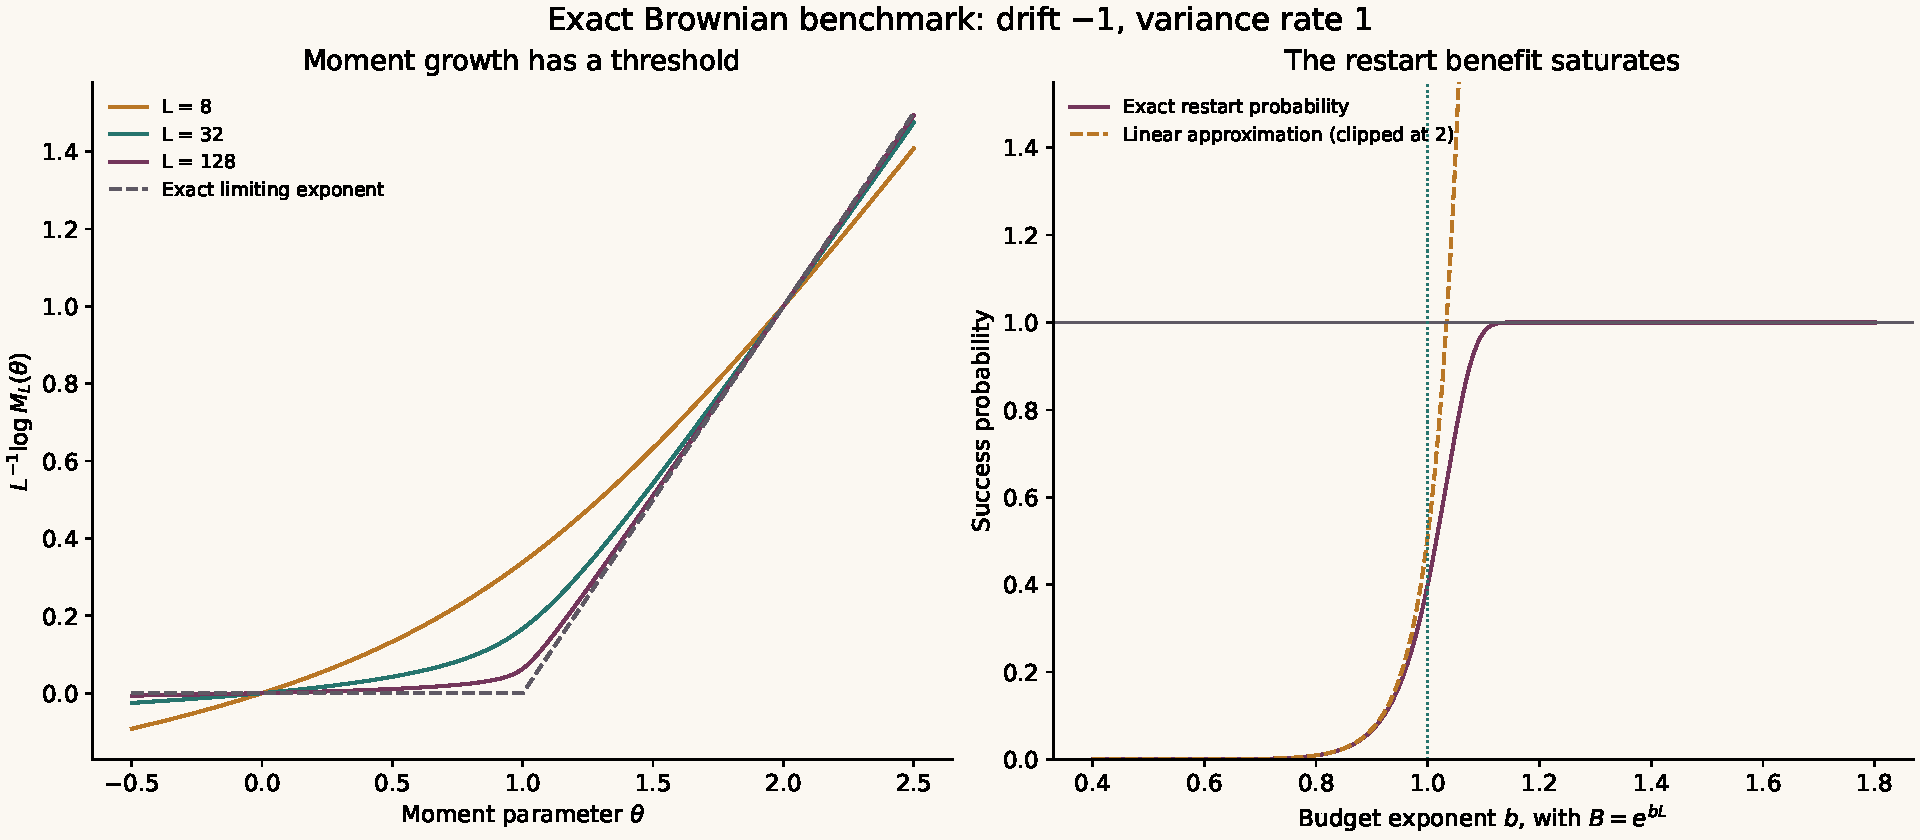
\includegraphics[width=\textwidth]{checks/moment_and_saturation.pdf}
\caption{Exact Brownian calculations ($m=\sigma=1$), not simulation. Left: the moment exponent $L^{-1}\log M_L(\theta)$ approaches $(\theta-\eta)_+$. Right ($L=20$): the restart success probability saturates once the budget passes $e^{\eta L}$, where the linear approximation leaves the range of probabilities.}
\label{fig:brownian}
\end{figure}

\subsection{The source's two-sided exponential-jump model}\label{sec:source}
The example of \cite[\S3.2.1]{garcia} has
\begin{equation}\label{eq:source-model}
 \psi(s)=-s+\frac{s^2}{2}-\frac{3s}{1+s}+\frac{2s}{4-s},\qquad -1<s<4,
\end{equation}
that is, unit Brownian part, drift $-1$, and L\'evy measure $\Pi(\dd y)=3e^{y}\dd y$ on $y<0$ plus $8e^{-4y}\dd y$ on $y>0$. Here $\lambda_*=2$ and
\[
 \eta=0.941150074276162\ldots,\qquad \kinf=1.337430736183531\ldots,\qquad v=2.379345600016397\ldots .
\]
The centred process has upward jumps with density $8e^{-\beta_+y}$, $\beta_+=4-\eta$, and downward jumps with density $3e^{\beta_-y}$ ($y<0$), $\beta_-=1+\eta$. Its cumulant factorises as
\[
 \chi(s)=\frac{s^2(a_+-s)(a_-+s)}{2(\beta_+-s)(\beta_-+s)},\qquad a_\pm=\mp\eta+\frac{(5-2\eta)\pm\sqrt{(5-2\eta)^2+32\kinf/\eta^2}}{2},
\]
with $a_+=4.42681549\ldots>\beta_+$ and $a_-=3.19141579\ldots>\beta_-$; the numerator $2(\beta_+-s)(\beta_-+s)\chi(s)=s^2(a_+-s)(a_-+s)$ shows directly why there are exactly two nonzero roots. The Wiener--Hopf factors are
\[
 \phi_+(q)=k_+\frac{q(q+a_+)}{q+\beta_+},\qquad \phi_-(q)=k_-\frac{q(q+a_-)}{q+\beta_-},\qquad k_+k_-=\tfrac12,
\]
legitimate drift-plus-compound-Poisson ladder exponents, with stationary overshoot transforms and means
\[
 G_\pm(s)=\frac{\beta_\pm(a_\pm-s)}{a_\pm(\beta_\pm-s)},\qquad \delta_\pm=\frac1{\beta_\pm}-\frac1{a_\pm},\qquad \delta_+=0.10102\ldots,\ \delta_-=0.20182\ldots
\]
The renewal profiles are explicit: $m_\pm V_\pm(y)=y+\delta_\pm(1-e^{-a_\pm y})$, which are the dashed curves in Figure~\ref{fig:layers}. Hence
\begin{equation}\label{eq:source-C}
\begin{aligned}
 C_*&=\frac{G_+(2-\eta)}{G_-(\eta)}=0.850148648990515392253315\ldots,\\
 R_*&=\kinf\frac{G_+(-\eta)}{G_-(\eta)}=0.906104425680893925439766\ldots
\end{aligned}
\end{equation}
These values are computed three ways (85-digit decimal arithmetic from the ladder and overshoot forms, and 70-digit arithmetic from formal boundary profiles) and enclosed by interval arithmetic (Proposition~\ref{prop:ratioone}(iv)); the swapped orientation would give $1.2926$ and $1.0255$.

\emph{Exact finite-interval solution.} Writing $p$ for the centred QSD density, the forward equation is a linear integro-differential equation with exponential kernels, which reduces to a fourth-order linear ODE. Its solutions are combinations of four exponentials $e^{s_jy}$, where $s_j$ solve a quartic: two fast real roots (one near $-a_+$, decaying from the left end, one near $a_-$, decaying from the right end) and a slow conjugate pair $\xi\pm i\omega$ with $\omega\approx\pi/L$. Four boundary conditions (the density vanishes at both ends, and the two jump-kernel integrals vanish at their entry ends) give a $4\times4$ linear system, whose determinant vanishes exactly at $\alpha=\alpha_L$. The moment and the restart rate follow from exact mode integrals and from the boundary fluxes (Gaussian flux plus the positive-jump exit intensity), independently of the constants \eqref{eq:source-C}. Table~\ref{tab:finiteL} gives the values in double precision (script \texttt{manuscript\_constant\_check.py}); the total exit flux matches $\kappa_L$ to better than $10^{-10}$ at every length. A high-precision version and the analysis of the $1/L$ terms are in \S\ref{sec:finiteL}.

\begin{table}[h]
\centering\small
\caption{Source model, exact finite-interval values. $C_L=e^{-(\lambda_*-\eta)L}M_L(\lambda_*)$, $R_L=e^{\eta L}r_L$. The last two columns show the first-order relative error $\approx0.50/L$ for both constants. ``Richardson'' is $2X_{1280}-X_{640}$.}\label{tab:finiteL}
\begin{tabular}{@{}rrrrrr@{}}
\toprule
$L$ & $L^2\alpha_L$ & $C_L$ & $R_L$ & $L(C_L/C_*-1)$ & $L(R_L/R_*-1)$\\
\midrule
40 & 11.558749 & 0.860517 & 0.922196 & 0.4879 & 0.710\\
80 & 11.651383 & 0.855385 & 0.912948 & 0.4927 & 0.604\\
160 & 11.696815 & 0.852779 & 0.909224 & 0.4951 & 0.551\\
320 & 11.719291 & 0.851467 & 0.907589 & 0.4963 & 0.524\\
640 & 11.730466 & 0.850809 & 0.906828 & 0.4968 & 0.511\\
1280 & 11.736039 & 0.850479 & 0.906461 & 0.4971 & 0.504\\
\midrule
Richardson & & 0.850149 & 0.906095 & &\\
Limit & 11.741600 & 0.850149 & 0.906104 & &\\
\bottomrule
\end{tabular}
\end{table}

\subsection{A non-reversible lattice diagnostic}
To test signs, orientation and the diffusive scaling outside the hypotheses, the script \texttt{verify.py} also treats a continuous-time lattice chain with jumps $+2$ at rate $1$, $+1$ at rate $1$ and $-1$ at rate $3$, killed outside $\{1,\ldots,n\}$. It is centred, non-reversible, has variance rate $8$, and has no Gaussian component, so it lies \emph{outside} Theorem~\ref{thm:main}. Exact rational arithmetic verifies the killed-matrix Esscher conjugacy for $n=2,\ldots,5$; for $n=255$ ($L=256$), $L^2\alpha_L=39.4007$ against $4\pi^2=39.4784$, and the QSD is within total variation $0.0013$ of the sampled sine law. Figure~\ref{fig:lattice} (Appendix~\ref{app:repro}) shows the convergence. This is a consistency diagnostic only.

%=====================================================================
\section{What the results mean for simulation practice}\label{sec:practice}
%=====================================================================
\emph{Budget rule.} For idealised QSD restart, Theorem~\ref{thm:restart} gives the budget for success probability $p$:
\begin{equation}\label{eq:budget-rule}
 B_p=\frac{-\log(1-p)}{r_L}\approx\frac{-\log(1-p)}{R_*}\,e^{\eta L},
\end{equation}
with relative error at most $|a_L-1|$ (about $0.5/L$ in the source model, \S\ref{sec:finiteL}). Below $e^{\eta L}$ success grows linearly in $B$; above it, extra budget buys almost nothing. Because the success time is exactly exponential (memoryless), no additional restart schedule layered on top of QSD restart can help, in line with the restart theory of Luby, Sinclair and Zuckerman \cite{lsz}.

\emph{Comparison of strategies.} Table~\ref{tab:cost} compares the order of the simulated time needed for a fixed success probability. Independent runs from $0$ (in parallel or in sequence) each succeed with probability about $C_{\mathrm{Cr}}e^{-\lambda_*L}$ provided each has length at least $(1+\varepsilon)L/\psi'(\lambda_*)$ \cite{garcia}, so they need total time of order $Le^{\lambda_*L}$. Idealised QSD restart needs order $e^{\eta L}$, an exponential gain $e^{(\lambda_*-\eta)L}$. Multilevel splitting and its adaptive and particle variants \cite{villen,ghsz,cerougu,cdgr,aldousvaz} place many intermediate levels between $0$ and $L$ and, under their standard conditions, reach a fixed relative accuracy with work that grows subexponentially in $L$. QSD restart is in effect a \emph{one-level} splitting scheme: it is exponentially better than independent runs and exponentially worse than well-designed multilevel methods. Its appeal is simplicity in model-free settings, the setting of \cite{garcia}. (The name RESTART in rare-event simulation \cite{villen} refers to a multilevel splitting method, not to the protocol studied here.)

\begin{table}[h]
\centering\small
\caption{Order of simulated time for a fixed success probability of reaching level $L$ (idealised, continuous monitoring).}\label{tab:cost}
\begin{tabularx}{\textwidth}{@{}p{.42\textwidth}Xl@{}}
\toprule
Strategy & Cost & Source of the rate\\
\midrule
Independent runs from $0$ (parallel or sequential) & $\asymp L\,e^{\lambda_*L}$ & Cram\'er; \cite{garcia,bertoindoney}\\
Idealised QSD restart (exact, free QSD draws) & $\sim-\log(1-p)\,e^{\eta L}/R_*$ & Theorem~\ref{thm:restart}\\
Multilevel splitting, AMS, Fleming--Viot with moving levels\textsuperscript{b} & subexponential in $L$ under standard conditions & \cite{ghsz,cerougu,cdgr}\\
\bottomrule
\end{tabularx}\\[2pt]
\raggedright\footnotesize\textsuperscript{b}\,For these methods the cost is that of producing weighted samples or an estimate of the rare-event probability with fixed relative accuracy, not of observing one unweighted path that reaches $L$; the row is not directly comparable with the first two.
\end{table}

\emph{The cost of sampling the QSD.} The theorem assumes exact, free draws from $\nu_L$. A natural implementation is a Fleming--Viot particle system \cite{bhm,ferrarimaric,villemonais14,afg} on $(0,L)$ started near the floor. Heuristically, the centred killed process relaxes to quasi-stationarity at the rate of the spectral gap, which the sine picture suggests is about $(4-1)\pi^2v/(2L^2)$; so a burn-in of order $L^2/v$ time units suffices, negligible against $e^{\eta L}$. After burn-in, $N$ particles produce upper exits at total rate about $Nr_L$, so the cost per success is again of order $e^{\eta L}/R_*$, up to a bias that vanishes as $N\to\infty$ \cite{villemonais14,cdgrfv}. With finitely many particles the success time is only approximately exponential. These statements are heuristic \status{exploratory}; the paper proves nothing about Fleming--Viot approximations. Note also that the idealised model would reward moving the floor upwards, which is unphysical: sampling a QSD close to the target is itself a rare-event problem. The natural design keeps the floor at the starting level.

\emph{Time discretisation.} The constants assume continuous monitoring. With a time step $\Delta t$, exits are detected late; for Brownian barriers the standard continuity correction shifts the barrier by about $0.5826\,\sigma\sqrt{\Delta t}$ \cite{bgk}, which changes the restart rate by a factor of roughly $e^{-0.5826\,\eta\sigma\sqrt{\Delta t}}$ (about $5\%$ for $\eta\approx0.94$, $\sigma=1$, $\Delta t=0.01$), comparable with the $15\%$ departure of $C_*$ from one in the source model. This is a heuristic order-of-magnitude statement for the Gaussian part only.

\emph{Model-free use.} In a model-free setting $\eta$, $\lambda_*$ and $R_*$ are unknown. Because cycle successes form an exact Poisson process in idealised restart, $r_L$ can be estimated by maximum likelihood from observed cycles at moderate $L$, and $\log r_L\approx\log R_*-\eta L+g_R/L$ extrapolates to larger $L$, with $g_R$ the first-order coefficient of \S\ref{sec:finiteL}.

%=====================================================================
\section{What remains open}\label{sec:open}
%=====================================================================
\begin{itemize}
\item \emph{Beyond the hypotheses.} Theorem~\ref{thm:sn} removes the Gaussian component for spectrally negative processes. For two-sided pure-jump processes, the proof uses $\sigma>0$ in four places: positive ladder drifts and the renewal bound $U_\pm\le d_\pm^{-1}\dd y$ (Lemma~\ref{lem:ladder}); the overshoot moment bounds (Lemma~\ref{lem:overshoot}); full support and the existence and uniqueness of the QSD (Remark~\ref{rem:support}); and the geometric bound on $\tau_L$ (Lemma~\ref{lem:exit}). Lattice and random-walk models, which the source also treats, raise arithmetic issues in the overshoot limits; the lattice diagnostic above is consistent with the sine law but proves nothing.
\item \emph{Finite-$L$ remainders.} Section~\ref{sec:finiteL} identifies the $1/L$ terms in the source model; the general statement (Conjecture~\ref{conj:general}) is open.
\item \emph{Implementable restart.} Quantitative bounds for Fleming--Viot or other approximate QSD sampling, charged restart overhead, and discrete monitoring require a separate analysis.
\item \emph{Random walks.} Whether the corrected budget range of Corollary~\ref{cor:corrected} holds for the random-walk case of \cite[Theorem 3.14]{garcia} is not addressed here.
\end{itemize}

\section*{Statements}
\paragraph{Use of AI tools.} Large language model-based AI tools were used extensively in developing the proofs, the computations and the text of this paper. The author has checked the results and takes full responsibility for the content. Every numerical statement can be regenerated with the accompanying code.
\paragraph{Data and code availability.} The scripts that generate every number, table and figure, together with their deterministic outputs, are available at \url{https://doi.org/10.5281/zenodo.23545672} (version 1.0.0-candidate; GitHub: \url{https://github.com/ipitchford/levy-qsd-exponential-moments-restart}). Appendix~\ref{app:repro} describes them.
\paragraph{Competing interests.} None.

\appendix
\section{Reproducibility}\label{app:repro}
Each script writes deterministic output (fixed rounding, no time stamps or version strings) and \texttt{verify\_all.py} reruns all of them into a temporary directory and compares the outputs byte for byte with the archived copies.
\begin{center}\small
\begin{tabularx}{\textwidth}{@{}lXl@{}}
\toprule
Script & What it checks & Label\\
\midrule
\texttt{verify.py} & Brownian identities, the counterexample \eqref{eq:counterexample}, rational lattice conjugacy, lattice diagnostics, Figures~\ref{fig:brownian} and~\ref{fig:lattice} & \status{certified}/\status{numerical}\\
\texttt{double\_exponential\_prefactor.py} & 70-digit factorisation of $\chi$ and two formulas for $C_*$ & \status{numerical}\\
\texttt{manuscript\_constant\_check.py} & 85-digit constants; exact finite-interval solution (Table~\ref{tab:finiteL}) & \status{numerical}\\
\texttt{e4\_ratio\_one.py} & interval enclosure of $C_*$, $R_*$; $C_*<1$ & \status{certified}\\
\texttt{e1\_effective\_length.py} & 70-digit finite-$L$ solution, $1/L$ and $L^{-2}$ coefficients (\S\ref{sec:finiteL}) & \status{numerical}\\
\texttt{e2\_spectrally\_negative.py} & scale-function computations for \S\ref{sec:sn} & \status{numerical}\\
\texttt{fig\_boundary\_layers.py} & Figure~\ref{fig:layers} & illustration\\
\bottomrule
\end{tabularx}
\end{center}
\begin{figure}[h]
\centering
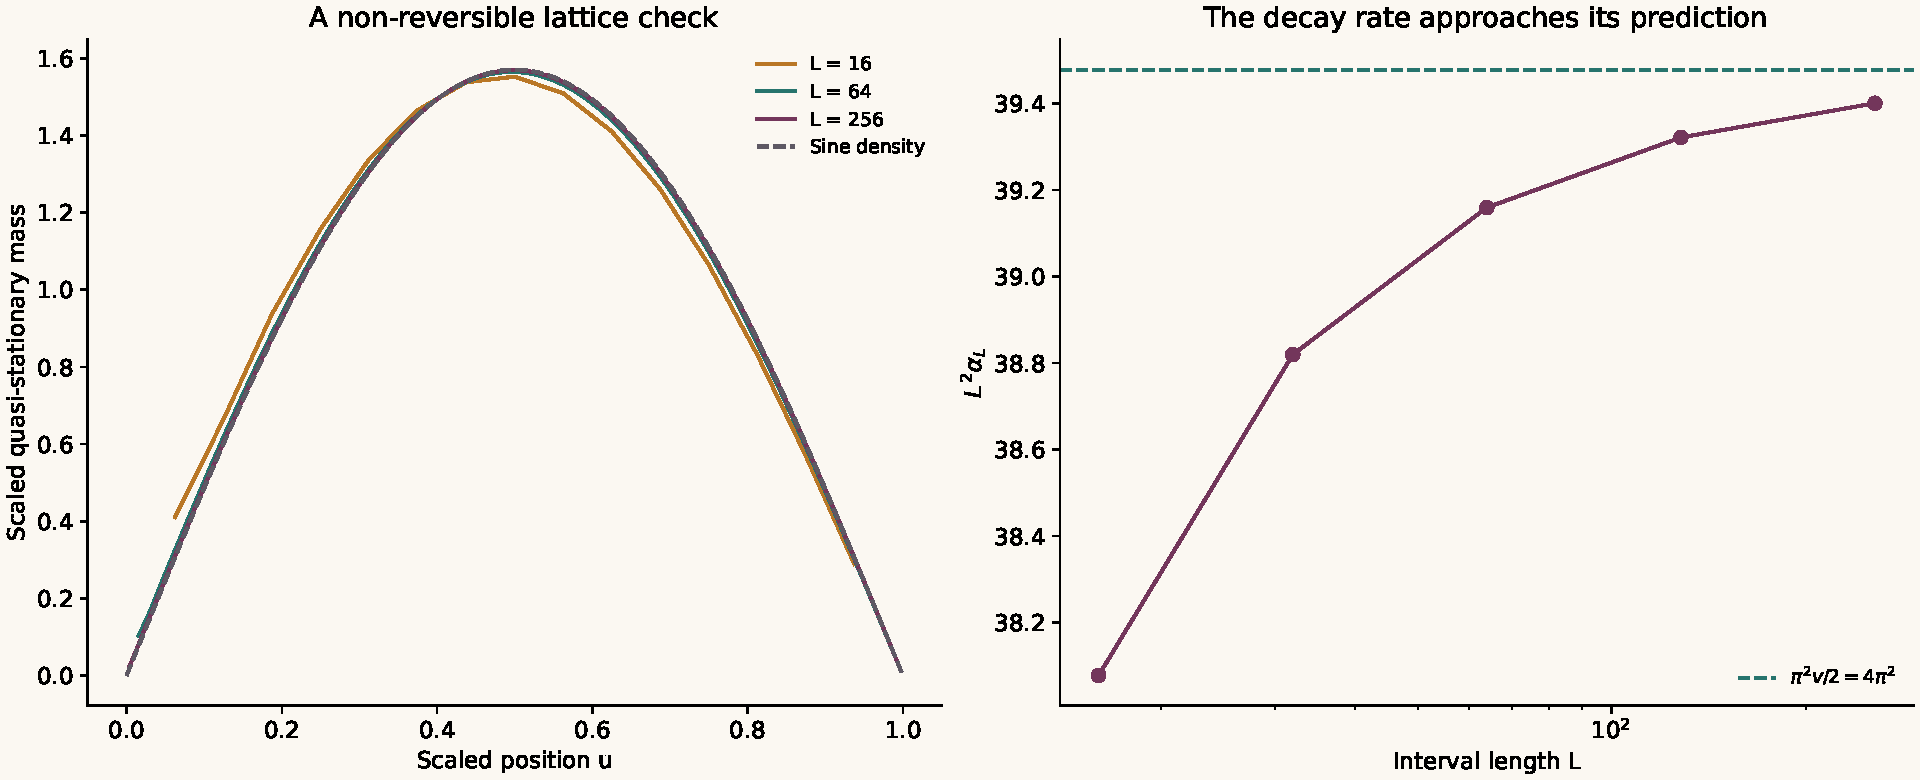
\includegraphics[width=\textwidth]{checks/lattice_scaling.pdf}
\caption{Non-reversible killed lattice chain (outside the hypotheses): the QSD approaches the sine profile and $L^2\alpha_L$ approaches $\pi^2v/2=4\pi^2$.}
\label{fig:lattice}
\end{figure}
\section{Interval certificate for $C_*<1$ in the source model}\label{app:cert}
This appendix makes Proposition~\ref{prop:ratioone}(iv) checkable from the paper. Multiplying $\psi'(s)$ by $(1+s)^2(4-s)^2>0$ gives the polynomial
\[
 P(s)=(s-1)(1+s)^2(4-s)^2-3(4-s)^2+8(1+s)^2,
\]
which has the sign of $\psi'(s)$ on $(-1,4)$; as $\psi'$ is strictly increasing there, $\eta$ is its unique zero. Exact rational bisection of $P$ on $[9/10,1]$ (200 steps) gives a rational isolating interval of width $2^{-200}/10$, contained in the decimal interval below. All other quantities are then evaluated in outward-rounded interval arithmetic (80 digits) from the formulas of \S\ref{sec:source}; every endpoint printed here is rounded outward to the digits shown (``$\ldots$'' repeats the digits of the lower endpoint).
\begin{center}\footnotesize
\begin{tabular}{@{}ll@{}}
\toprule
Quantity & Enclosure\\
\midrule
$\eta$ & $[0.941150074276162503617693510244547522143206347,\ \ldots348]$\\
$\kinf$ & $[1.3374307361835312965316735595491422761236,\ \ldots237]$\\
$\beta_+=4-\eta$ & $[3.0588499257238374963823064897554524778567,\ \ldots568]$\\
$\beta_-=1+\eta$ & $[1.9411500742761625036176935102445475221432,\ \ldots433]$\\
$a_+$ & $[4.4268154934824107937849738546480267651465,\ \ldots466]$\\
$a_-$ & $[3.1914157905870608082557478956262168537193,\ \ldots194]$\\
$G_+(\lambda_*-\eta)$ & $[1.1636018309263749054473691808046099876611,\ \ldots612]$\\
$G_-(\eta)$ & $[1.3687039699563840931584374388704957674053,\ \ldots054]$\\
$G_+(-\eta)$ & $[0.9272919270297836291448413417853360614948,\ \ldots949]$\\
$C_*$ & $[0.8501486489905153922533152069617579603498,\ \ldots499]$\\
$R_*$ & $[0.9061044256808939254397660894952892493141,\ \ldots142]$\\
\bottomrule
\end{tabular}
\end{center}
In particular $a_+>\beta_+$ and $a_->\beta_-$, as required for the ladder factors to be Bernstein functions, and $C_*<1$. The script also evaluates $\chi(s)$ minus its rational factorisation at four points; this is a consistency test of the transcription, not part of the certificate, since the factorisation is exact algebra. Script: \texttt{e4\_ratio\_one.py}; output \texttt{checks/e4\_ratio\_one.json}.

\begin{thebibliography}{99}

\bibitem{aldousvaz}
Aldous, D. and Vazirani, U. (1994). ``Go with the winners'' algorithms. In \emph{Proceedings 35th Annual Symposium on Foundations of Computer Science (FOCS)}, pp.~492--501. IEEE. \url{https://doi.org/10.1109/SFCS.1994.365742}

\bibitem{afg}
Asselah, A., Ferrari, P.~A. and Groisman, P. (2011). Quasistationary distributions and Fleming--Viot processes in finite spaces. \emph{Journal of Applied Probability, 48}(2), 322--332. \url{https://doi.org/10.1239/jap/1308662630}

\bibitem{aap}
Asmussen, S., Avram, F. and Pistorius, M.~R. (2004). Russian and American put options under exponential phase-type L\'evy models. \emph{Stochastic Processes and their Applications, 109}(1), 79--111. \url{https://doi.org/10.1016/j.spa.2003.07.005}

\bibitem{bertoinbook}
Bertoin, J. (1996). \emph{L\'evy Processes}. Cambridge Tracts in Mathematics, Vol.~121. Cambridge University Press, Cambridge. ISBN 0-521-56243-0.

\bibitem{bertoin97}
Bertoin, J. (1997). Exponential decay and ergodicity of completely asymmetric L\'evy processes in a finite interval. \emph{The Annals of Applied Probability, 7}(1), 156--169. \url{https://doi.org/10.1214/aoap/1034625257}

\bibitem{bertoindoney}
Bertoin, J. and Doney, R.~A. (1994). Cram\'er's estimate for L\'evy processes. \emph{Statistics \& Probability Letters, 21}(5), 363--365. \url{https://doi.org/10.1016/0167-7152(94)00032-8}

\bibitem{bvhs}
Bertoin, J., van Harn, K. and Steutel, F.~W. (1999). Renewal theory and level passage by subordinators. \emph{Statistics \& Probability Letters, 45}(1), 65--69. \url{https://doi.org/10.1016/S0167-7152(99)00043-7}

\bibitem{bgk}
Broadie, M., Glasserman, P. and Kou, S. (1997). A continuity correction for discrete barrier options. \emph{Mathematical Finance, 7}(4), 325--349. \url{https://doi.org/10.1111/1467-9965.00035}

\bibitem{bhm}
Burdzy, K., Ho{\l}yst, R. and March, P. (2000). A Fleming--Viot particle representation of the Dirichlet Laplacian. \emph{Communications in Mathematical Physics, 214}(3), 679--703. \url{https://doi.org/10.1007/s002200000294}

\bibitem{cerougu}
C\'erou, F. and Guyader, A. (2007). Adaptive multilevel splitting for rare event analysis. \emph{Stochastic Analysis and Applications, 25}(2), 417--443. \url{https://doi.org/10.1080/07362990601139628}

\bibitem{cdgr}
C\'erou, F., Delyon, B., Guyader, A. and Rousset, M. (2019). On the asymptotic normality of adaptive multilevel splitting. \emph{SIAM/ASA Journal on Uncertainty Quantification, 7}(1), 1--30. \url{https://doi.org/10.1137/18M1187477}

\bibitem{cdgrfv}
C\'erou, F., Delyon, B., Guyader, A. and Rousset, M. (2020). A central limit theorem for Fleming--Viot particle systems. \emph{Annales de l'Institut Henri Poincar\'e, Probabilit\'es et Statistiques, 56}(1), 637--666. \url{https://doi.org/10.1214/19-AIHP976}

\bibitem{champvill}
Champagnat, N. and Villemonais, D. (2016). Exponential convergence to quasi-stationary distribution and $Q$-process. \emph{Probability Theory and Related Fields, 164}(1--2), 243--283. \url{https://doi.org/10.1007/s00440-014-0611-7}

\bibitem{cms}
Collet, P., Mart\'inez, S. and San Mart\'in, J. (2013). \emph{Quasi-Stationary Distributions: Markov Chains, Diffusions and Dynamical Systems}. Probability and Its Applications. Springer, Berlin. \url{https://doi.org/10.1007/978-3-642-33131-2}

\bibitem{denisovshneer}
Denisov, D. and Shneer, V. (2013). Asymptotics for the first passage times of L\'evy processes and random walks. \emph{Journal of Applied Probability, 50}(1), 64--84. \url{https://doi.org/10.1239/jap/1363784425}

\bibitem{doney}
Doney, R.~A. (2007). \emph{Fluctuation Theory for L\'evy Processes}. Ecole d'\'Et\'e de Probabilit\'es de Saint-Flour XXXV--2005 (J.~Picard, ed.). Lecture Notes in Mathematics, Vol.~1897. Springer, Berlin. \url{https://doi.org/10.1007/978-3-540-48511-7}

\bibitem{doring}
D\"oring, L. and Trottner, L. (2023). Stability of overshoots of Markov additive processes. \emph{The Annals of Applied Probability, 33}(6B), 5413--5458. \url{https://doi.org/10.1214/23-AAP1951}. Theorem numbers cited refer to the authors' accepted manuscript; in arXiv:2102.03238v2 the corresponding results are Theorems 3.10, 3.18, 4.3 and Proposition 3.16.

\bibitem{du}
Du, Y., Fang, X. and Ni, W. (2025). Asymptotic limit of the principal eigenvalue of asymmetric nonlocal diffusion operators and propagation dynamics. Preprint, arXiv:2503.22062v2 (20 August 2025). \url{https://arxiv.org/abs/2503.22062}

\bibitem{goexplore}
Ecoffet, A., Huizinga, J., Lehman, J., Stanley, K.~O. and Clune, J. (2021). First return, then explore. \emph{Nature, 590}(7847), 580--586. \url{https://doi.org/10.1038/s41586-020-03157-9}

\bibitem{evansmaj}
Evans, M.~R. and Majumdar, S.~N. (2011). Diffusion with stochastic resetting. \emph{Physical Review Letters, 106}(16), 160601. \url{https://doi.org/10.1103/PhysRevLett.106.160601}

\bibitem{ferrarimaric}
Ferrari, P.~A. and Mari\'c, N. (2007). Quasi stationary distributions and Fleming--Viot processes in countable spaces. \emph{Electronic Journal of Probability, 12}, 684--702. \url{https://doi.org/10.1214/EJP.v12-415}

\bibitem{garcia}
Garcia, E., Bermolen, P., Jonckheere, M. and Shneer, S. (2026). Efficiency of parallel and restart exploration strategies in model-free stochastic simulations. \emph{Stochastic Systems, 16}(3), 264--288. \url{https://doi.org/10.1287/stsy.2025.0108}. Preprint arXiv:2503.03565v3 (6 May 2026).

\bibitem{garciarossi}
Garc\'ia-Meli\'an, J. and Rossi, J.~D. (2009). On the principal eigenvalue of some nonlocal diffusion problems. \emph{Journal of Differential Equations, 246}(1), 21--38. \url{https://doi.org/10.1016/j.jde.2008.04.015}

\bibitem{ghsz}
Glasserman, P., Heidelberger, P., Shahabuddin, P. and Zajic, T. (1999). Multilevel splitting for estimating rare event probabilities. \emph{Operations Research, 47}(4), 585--600. \url{https://doi.org/10.1287/opre.47.4.585}

\bibitem{grzywny}
Grzywny, T. (2019). First exit times from a bounded interval for L\'evy processes. Preprint, arXiv:1911.05022v1 (12 November 2019). \url{https://arxiv.org/abs/1911.05022}

\bibitem{kadver}
Kadankova, T. and Veraverbeke, N. (2007). On several two-boundary problems for a particular class of L\'evy processes. \emph{Journal of Theoretical Probability, 20}(4), 1073--1085. \url{https://doi.org/10.1007/s10959-007-0088-8}

\bibitem{khodzhibaev14}
Khodzhibaev, V.~R. (2014). \emph{Ob asimptotike raspredelenii, svyazannykh s vykhodom sluchainogo protsessa s nezavisimymi prirashcheniyami iz intervala} [On the asymptotics of distributions related to the exit of a process with independent increments from an interval]. Fan va texnologiya, Tashkent. ISBN 978-9943-4349-3-6. (In Russian.)

\bibitem{kolbsavov}
Kolb, M. and Savov, M. (2014). Exponential ergodicity of killed L\'evy processes in a finite interval. \emph{Electronic Communications in Probability, 19}, paper no.~31, 1--9. \url{https://doi.org/10.1214/ECP.v19-3006}

\bibitem{kolbst}
Kolb, M. and Steinsaltz, D. (2012). Quasilimiting behavior for one-dimensional diffusions with killing. \emph{The Annals of Probability, 40}(1), 162--212. \url{https://doi.org/10.1214/10-AOP623}

\bibitem{kyprianoubook}
Kyprianou, A.~E. (2014). \emph{Fluctuations of L\'evy Processes with Applications: Introductory Lectures} (2nd ed.). Universitext. Springer, Berlin. \url{https://doi.org/10.1007/978-3-642-37632-0}

\bibitem{kypalm}
Kyprianou, A.~E. and Palmowski, Z. (2006). Quasi-stationary distributions for L\'evy processes. \emph{Bernoulli, 12}(4), 571--581. \url{https://doi.org/10.3150/bj/1155735927}

\bibitem{lambert}
Lambert, A. (2000). Completely asymmetric L\'evy processes confined in a finite interval. \emph{Annales de l'Institut Henri Poincar\'e, Probabilit\'es et Statistiques, 36}(2), 251--274. \url{https://doi.org/10.1016/S0246-0203(00)00126-6}

\bibitem{lotov79}
Lotov, V.~I. (1979). Asymptotic analysis of distributions in problems with two boundaries. I, II. \emph{Teoriya Veroyatnostei i ee Primeneniya, 24}(3), 475--485; 24(4), 873--879. English transl.: \emph{Theory of Probability and Its Applications, 24}(3), 480--491 (1980), \url{https://doi.org/10.1137/1124059}; 24(4), 869--876 (1980), \url{https://doi.org/10.1137/1124103}

\bibitem{lotov16}
Lotov, V.~I. (2016). Approximation of the expectation of the first exit time from an interval for a random walk. \emph{Siberian Mathematical Journal, 57}(1), 86--92. \url{https://doi.org/10.1134/S0037446616010092}

\bibitem{lotovkh}
Lotov, V.~I. and Khodzhibaev, V.~R. (1998). On limit theorems for the first exit time from an interval for stochastic processes. I. \emph{Matematicheskie Trudy, 1}(2), 111--134. English transl.: \emph{Siberian Advances in Mathematics, 8}(3), 90--113 (1998). Part II: \emph{Mat.\ Trudy, 2}(1), 121--139 (1999); English transl.\ \emph{Sib.\ Adv.\ Math., 8}(4), 41--59 (1998).

\bibitem{lsz}
Luby, M., Sinclair, A. and Zuckerman, D. (1993). Optimal speedup of Las Vegas algorithms. \emph{Information Processing Letters, 47}(4), 173--180. \url{https://doi.org/10.1016/0020-0190(93)90029-9}

\bibitem{mandl}
Mandl, P. (1961). Spectral theory of semi-groups connected with diffusion processes and its application. \emph{Czechoslovak Mathematical Journal, 11}(4), 558--569. \url{https://doi.org/10.21136/CMJ.1961.100484}

\bibitem{martinezsm}
Mart\'inez, S. and San Mart\'in, J. (1994). Quasi-stationary distributions for a Brownian motion with drift and associated limit laws. \emph{Journal of Applied Probability, 31}(4), 911--920. \url{https://doi.org/10.2307/3215316}

\bibitem{melvill}
M\'el\'eard, S. and Villemonais, D. (2012). Quasi-stationary distributions and population processes. \emph{Probability Surveys, 9}, 340--410. \url{https://doi.org/10.1214/11-PS191}

\bibitem{palreuveni}
Pal, A. and Reuveni, S. (2017). First passage under restart. \emph{Physical Review Letters, 118}(3), 030603. \url{https://doi.org/10.1103/PhysRevLett.118.030603}

\bibitem{ponomarev}
Ponomarev, D. (2021). Asymptotic solution to convolution integral equations on large and small intervals. \emph{Proceedings of the Royal Society A, 477}(2248), 20210025. \url{https://doi.org/10.1098/rspa.2021.0025}

\bibitem{vigon}
Vigon, V. (2002). \emph{Simplifiez vos L\'evy en titillant la factorisation de Wiener--Hopf}. Th\`ese de doctorat, INSA de Rouen (dir.\ S.~Fourati). theses.fr NNT 2002ISAM0002; HAL tel-00567466. \url{https://theses.hal.science/tel-00567466}

\bibitem{villemonais14}
Villemonais, D. (2014). General approximation method for the distribution of Markov processes conditioned not to be killed. \emph{ESAIM: Probability and Statistics, 18}, 441--467. \url{https://doi.org/10.1051/ps/2013045}

\bibitem{villen}
Vill\'en-Altamirano, M. and Vill\'en-Altamirano, J. (1994). RESTART: a straightforward method for fast simulation of rare events. In \emph{Proceedings of the 1994 Winter Simulation Conference}, pp.~282--289. IEEE. \url{https://doi.org/10.1109/WSC.1994.717150}

\bibitem{zbik}
Zbik, B. and Palmowski, Z. (2026). Asymptotic behaviour for escaping an interval by L\'evy flights under stochastic resetting. Preprint, arXiv:2610.20410v1 (14 October 2026). \url{https://arxiv.org/abs/2610.20410}

\end{thebibliography}

\end{document}
